\documentclass[12pt,a4paper]{article}

% ------------------------------------------------------------------
% Formato APA 7 (trabajo de estudiante)
% ------------------------------------------------------------------
\usepackage[utf8]{inputenc}
\usepackage[T1]{fontenc}
\usepackage[spanish,es-tabla,es-nodecimaldot]{babel}
\usepackage{mathptmx}                 % Times New Roman (texto y matemáticas)
\usepackage{microtype}
\usepackage[margin=2.54cm]{geometry}  % márgenes de 1 pulgada
\usepackage{setspace}
\doublespacing                        % doble espacio
\usepackage{amsmath,amssymb,bm}
\usepackage{graphicx}
\usepackage{booktabs}
\usepackage{tabularx}
\usepackage{float}
\usepackage{caption}
\usepackage{enumitem}
\usepackage{fancyhdr}
\usepackage{titlesec}
\usepackage[round,authoryear]{natbib}
\usepackage[hidelinks]{hyperref}
\usepackage{url}
\urlstyle{same}

\graphicspath{{../figuras/}{./}}

% Sangría de primera línea de 1,27 cm
\setlength{\parindent}{1.27cm}
\setlength{\parskip}{0pt}

% Títulos APA: sin numeración
\setcounter{secnumdepth}{0}
% Nivel 1: centrado, negrita
\titleformat{\section}{\normalsize\bfseries\filcenter}{}{0pt}{}
% Nivel 2: alineado a la izquierda, negrita
\titleformat{\subsection}{\normalsize\bfseries}{}{0pt}{}
% Nivel 3: alineado a la izquierda, negrita cursiva
\titleformat{\subsubsection}{\normalsize\bfseries\itshape}{}{0pt}{}
% Nivel 4: con sangría, negrita, termina en punto, texto en la misma línea
\titleformat{\paragraph}[runin]{\normalsize\bfseries}{}{0pt}{\hspace*{1.27cm}}[]
\titlespacing*{\section}{0pt}{12pt}{0pt}
\titlespacing*{\subsection}{0pt}{12pt}{0pt}
\titlespacing*{\subsubsection}{0pt}{12pt}{0pt}
\titlespacing*{\paragraph}{0pt}{0pt}{0.5em}

% Tablas y figuras APA: número en negrita, título en cursiva en la línea siguiente, ambos arriba
\captionsetup{labelfont=bf,textfont=it,labelsep=newline,justification=raggedright,
  singlelinecheck=false,font={normalsize,singlespacing},skip=6pt}
\newcommand{\nota}[1]{\par\vspace{4pt}{\setstretch{1}\small\raggedright\textit{Nota.} #1\par}}

% Encabezado: solo número de página arriba a la derecha
\pagestyle{fancy}
\fancyhf{}
\fancyhead[R]{\thepage}
\renewcommand{\headrulewidth}{0pt}

% Listas con el mismo interlineado
\setlist{itemsep=0pt,topsep=2pt,parsep=0pt}

% Referencias: sangría francesa de 1,27 cm
\setlength{\bibhang}{1.27cm}
\setlength{\bibsep}{0pt}
\renewcommand{\bibsection}{\section{Referencias}}

\newcommand{\lnC}{\ln(\text{Confirmed}+1)}
\newcommand{\lnD}{\ln(\text{Deaths}+1)}

\begin{document}

% ------------------------------ Portada ------------------------------
\begin{titlepage}
\thispagestyle{fancy}
\centering
\vspace*{0.4cm}

\includegraphics[width=2.8cm]{logo_unmsm.png}\par
\vspace{1cm}
{\bfseries Difusión Global y Estimación Espacial del COVID-19:\\
Análisis Geoestadístico en Europa con Kriging y Cokriging\par}
\vspace{1cm}
Grupo 6\par
\vspace{0.2cm}
{\setstretch{1.3}
\begin{tabular}{lc}
\toprule
Apellidos y nombres & Participación \\
\midrule
Briceño Ypanaque, Gabriel & 100\,\% \\
Espinoza Luna, Wilder & 100\,\% \\
Isase Camara, Vicente & 100\,\% \\
Montoya Juro, Oscar & 100\,\% \\
Pablo Machaca, Gerson & 100\,\% \\
Polastre Mamani, Frank & 100\,\% \\
\bottomrule
\end{tabular}\par}
\vspace{0.8cm}
Escuela Profesional de Estadística, Facultad de Ciencias Matemáticas\par
Universidad Nacional Mayor de San Marcos\par
Estadística Espacial: Segunda Práctica Calificada\par
Dr. Misael Erikson Maguiña Palma\par
17 de noviembre de 2026\par
\end{titlepage}
\setcounter{page}{2}

% ------------------------------ Resumen ------------------------------
\section{Resumen}
\noindent Se modeló la distribución espacial de los casos confirmados y de las defunciones por COVID-19 en la Región Europa de la Organización Mundial de la Salud al 26 de julio de 2020, a partir de 52 puntos de reporte integrados con indicadores demográficos y sanitarios de Our World in Data. La proyección a ETRS89-LAEA (EPSG:3035) redujo el error de distancia frente a la geodésica de una mediana de 29,9\,\% a un máximo de 2,1\,\%. Tras la transformación $\ln(x+1)$ y la homogeneización del soporte espacial, la proporción pepita/meseta descendió de 61,7\,\% a 23,3\,\%. El patrón de sitios rechazó la hipótesis de Completa Aleatoriedad Espacial ($R=1{,}35$, $p<0{,}001$; contraste MAD, $p=0{,}020$). El semivariograma de los casos, estimado por máxima verosimilitud y seleccionado por validación cruzada, correspondió a un modelo gaussiano sin efecto pepita y con alcance práctico de 393\,km. El Kriging Ordinario superó al interpolador IDW (RMSE de 1,583 frente a 1,655) con varianza calibrada (RMSS $=1{,}02$). Bajo un Modelo Lineal de Corregionalización admisible, el Cokriging Ordinario coincidió con el Kriging en muestreo isotópico y redujo el RMSE en 66\,\% cuando la variable secundaria estuvo disponible en el sitio de predicción. Los resultados sustentan tres recomendaciones cuantificadas sobre capacidad hospitalaria, densidad de vigilancia y coordinación territorial.

\par\hspace*{1.27cm}\textit{Palabras clave:} geoestadística, semivariograma, Kriging Ordinario, Cokriging, corregionalización, procesos puntuales, COVID-19
\clearpage

% ------------------------------ Introducción ------------------------------
\begin{center}\textbf{Difusión Global y Estimación Espacial del COVID-19: Análisis Geoestadístico en Europa con Kriging y Cokriging}\end{center}

La propagación del SARS-CoV-2 durante la primera ola de la pandemia, entre enero y julio de 2020, presentó una marcada heterogeneidad espacial en Europa. La proximidad geográfica, la movilidad transfronteriza y las decisiones nacionales de contención configuraron un mapa epidemiológico desigual cuya descripción requiere métodos que reconozcan la dependencia entre observaciones cercanas. La estadística espacial proporciona dicho marco: permite describir la estructura de la variabilidad, cuantificar la dependencia en función de la distancia y predecir la variable de interés en localizaciones no observadas con una medida explícita de incertidumbre \citep{cressie1993,diggle1998}.

El presente estudio emplea el conjunto de datos \emph{Data Spatial}, compilado a partir de la serie diaria del Centro de Ciencia e Ingeniería de Sistemas de la Universidad Johns Hopkins \citep{dong2020}. El conjunto contiene 49\,068 registros correspondientes a 261 ubicaciones y 188 fechas, del 22 de enero al 26 de julio de 2020, con las variables casos confirmados (Confirmed), defunciones (Deaths), recuperados (Recovered) y activos (Active), las coordenadas geográficas de cada ubicación en el sistema WGS84 y la región de la Organización Mundial de la Salud (OMS) a la que pertenece.

El objetivo general es modelar la distribución espacial de los casos confirmados y de las defunciones por COVID-19 en Europa al 26 de julio de 2020 mediante métodos geoestadísticos, con el fin de obtener superficies continuas de propagación y mapas de incertidumbre que orienten la asignación de recursos sanitarios. Los objetivos específicos son (a) preparar y proyectar los datos y justificar el corte temporal y la transformación de las variables; (b) caracterizar el patrón de los sitios de reporte e interpolar con el método del inverso de la distancia; (c) modelar la dependencia espacial mediante semivariogramas, estimar por Kriging Ordinario y Cokriging Ordinario y seleccionar el estimador mediante validación cruzada; y (d) traducir las superficies estimadas y su incertidumbre en recomendaciones territoriales cuantificadas. La correspondencia entre las secciones del informe y los ítems de la práctica se presenta en el Apéndice A.

\section{Método}

\subsection{Datos y Fuentes Complementarias}

El conjunto \emph{Data Spatial} se lee de forma automatizada desde el repositorio público del proyecto en GitHub (\url{https://github.com/wilder1111/BI1/blob/main/Data%20Spatial.csv}), con una copia local de respaldo para ejecuciones sin conexión. Además, se integraron dos fuentes abiertas mediante el nombre del país. De Our World in Data \citep{owid2020} se obtuvieron la población, la densidad poblacional, el porcentaje de población de 65 años o más y el número de camas hospitalarias por cada 1000 habitantes, con referencia al 26 de julio de 2020. De Natural Earth \citep{naturalearth} se obtuvieron los polígonos de fronteras nacionales a escala 1:50\,000\,000, que se emplearon como máscara de interpolación y como ventana de observación del proceso puntual.

\subsection{Procedimiento Computacional}

El análisis se implementó en Python con las bibliotecas \texttt{geopandas}, \texttt{pyproj}, \texttt{numpy}, \texttt{scipy}, \texttt{statsmodels} y PySAL/\texttt{esda} \citep{rey2007}. Los sistemas de Kriging Ordinario, Kriging Universal y Cokriging Ordinario se programaron en forma matricial para hacer explícitas sus ecuaciones, y la implementación del Kriging Ordinario se verificó contra la biblioteca \texttt{pykrige}. Se fijó la semilla aleatoria 2020 para garantizar la reproducibilidad de las simulaciones y permutaciones. El código completo se encuentra en un único cuaderno Jupyter (Apéndice B).

% =====================================================================
\section{Fase 1: Preparación, Tratamiento Espacial y Geoprocesamiento}
% =====================================================================

\subsection{Sesgo de la Distancia Euclidiana en Coordenadas Geográficas}

Las coordenadas $(\lambda,\varphi)$ del sistema WGS84 (EPSG:4326) son ángulos sobre un elipsoide y no posiciones en un plano. En consecuencia, la distancia
\[
d_{\deg}(s_i,s_j)=\sqrt{(\lambda_i-\lambda_j)^2+(\varphi_i-\varphi_j)^2}
\]
carece de significado métrico y sesga el semivariograma empírico de la variable Confirmed por cuatro vías. En primer lugar, la convergencia de los meridianos introduce una anisotropía artificial: un grado de latitud equivale aproximadamente a 111,3\,km en todo el globo, mientras que un grado de longitud equivale a $111{,}32\cos\varphi$\,km, es decir, 90,1\,km a 36\,°N y 38,1\,km a 70\,°N. Separaciones físicas que difieren en más del doble reciben, por tanto, el mismo valor de $d_{\deg}$. En segundo lugar, el estimador de Matheron agrupa los pares de observaciones por clases de distancia; si estas se definen en grados, una misma clase combina pares cercanos situados en latitudes altas con pares lejanos situados en latitudes bajas, de modo que $\hat\gamma(h)$ queda sesgado de forma sistemática según la latitud.

En tercer lugar, se vulnera la hipótesis de estacionariedad intrínseca, según la cual $\operatorname{Var}[Z(s+h)-Z(s)]=2\gamma(h)$ depende únicamente del vector de separación $h$: un mismo incremento angular representa distancias diferentes en distintas latitudes. Por último, los parámetros del modelo pierden significado físico, porque el alcance quedaría expresado en una unidad no constante, y la admisibilidad de los modelos esférico, exponencial y gaussiano, que son condicionalmente definidos negativos en $\mathbb R^2$ con la distancia euclidiana, deja de estar garantizada; las varianzas de Kriging resultan, en consecuencia, mal calibradas \citep{chiles2012}.

La magnitud del sesgo se cuantificó sobre los 1326 pares de puntos del área de estudio, tomando como referencia la distancia geodésica sobre el elipsoide WGS84 (Tabla~\ref{tab:dist} y Figura~\ref{fig:dist}). La distancia en grados presentó un error relativo mediano de 29,9\,\% y un error máximo de 125,9\,\%, con un patrón creciente en función de la latitud que confirma el carácter sistemático, y no aleatorio, de la distorsión.

\begin{table}[H]\centering\setstretch{1}\small
\caption{Error Relativo de la Distancia Calculada Frente a la Distancia Geodésica}\label{tab:dist}
\begin{tabular}{lccc}\toprule
Métrica & Error mediano (\%) & $|$Error$|$ P95 (\%) & $|$Error$|$ máximo (\%)\\\midrule
Euclidiana en grados ($\times$111,32 km) & 29,87 & 61,28 & 125,92\\
Euclidiana en EPSG:3035 & $-0{,}07$ & 0,72 & 2,06\\\bottomrule
\end{tabular}
\nota{Cálculo sobre los 1326 pares de las 52 ubicaciones del área de estudio. P95 = percentil 95. Elaboración propia a partir de \citet{dong2020}.}
\end{table}

\begin{figure}[H]
\caption{Distancia Calculada Frente a la Distancia Geodésica, Según Latitud Media del Par}\label{fig:dist}
\centering
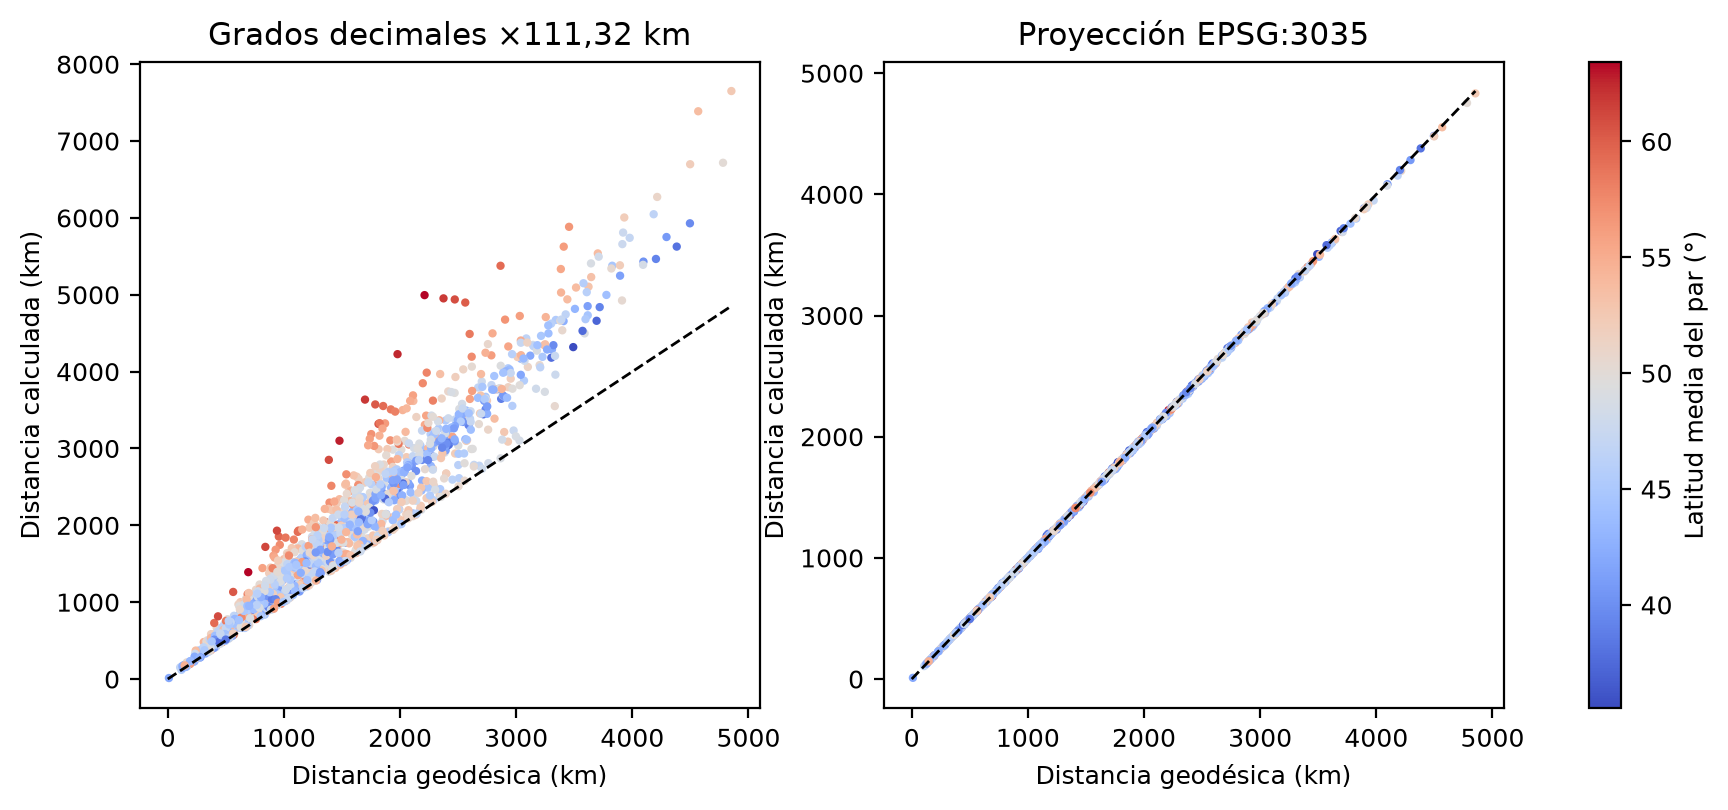
\includegraphics[width=0.9\linewidth]{f1_distancias_grados_vs_proyectadas.png}
\nota{El panel izquierdo emplea grados decimales y el derecho la proyección EPSG:3035. La línea discontinua representa la igualdad entre ambas distancias. Elaboración propia.}
\end{figure}

\subsection{Sistema de Coordenadas Proyectadas Propuesto}

Para el análisis geoestadístico de la Región Europa se propone la proyección Azimutal Equivalente de Lambert sobre el datum ETRS89, centrada en 52\,°N y 10\,°E y con unidades en metros (ETRS89/LAEA Europe, EPSG:3035). Esta proyección es la referencia oficial de la Unión Europea para el análisis estadístico paneuropeo y la base de su grilla estadística \citep{annoni2003}. Su carácter equivalente conserva las áreas, propiedad necesaria para estimar intensidades de procesos puntuales, y su carácter azimutal, centrado en el continente, mantiene reducida la distorsión de distancias en toda la región \citep{snyder1987}; en los datos analizados, el error máximo fue de 2,06\,\% (Tabla~\ref{tab:dist}). Se descartaron el sistema UTM, cuyos husos de 6° impiden disponer de un plano común para un territorio que abarca más de diez husos, y la proyección Web Mercator (EPSG:3857), cuyo factor de escala $\sec\varphi$ exagera las distancias en más de 100\,\% en Escandinavia. Para la región del Pacífico Occidental, que carece de un código EPSG continental equivalente, correspondería definir una proyección azimutal equidistante centrada en la región, que conserva exactamente las distancias desde el punto central.

Dado que la Región Europa de la OMS incluye territorios de ultramar y países de Asia Central, el análisis se restringió a la ventana comprendida entre 25\,°O y 46\,°E de longitud y entre 34\,°N y 72\,°N de latitud, correspondiente a la zona de validez de EPSG:3035. Dicha ventana contiene 52 de las 80 ubicaciones de la región (Figura~\ref{fig:puntos}). La Federación de Rusia quedó excluida debido a que su centroide se localiza en 105\,°E.

\begin{figure}[H]
\caption{Localización de los Puntos de Reporte en EPSG:3035 al 26 de Julio de 2020}\label{fig:puntos}
\centering
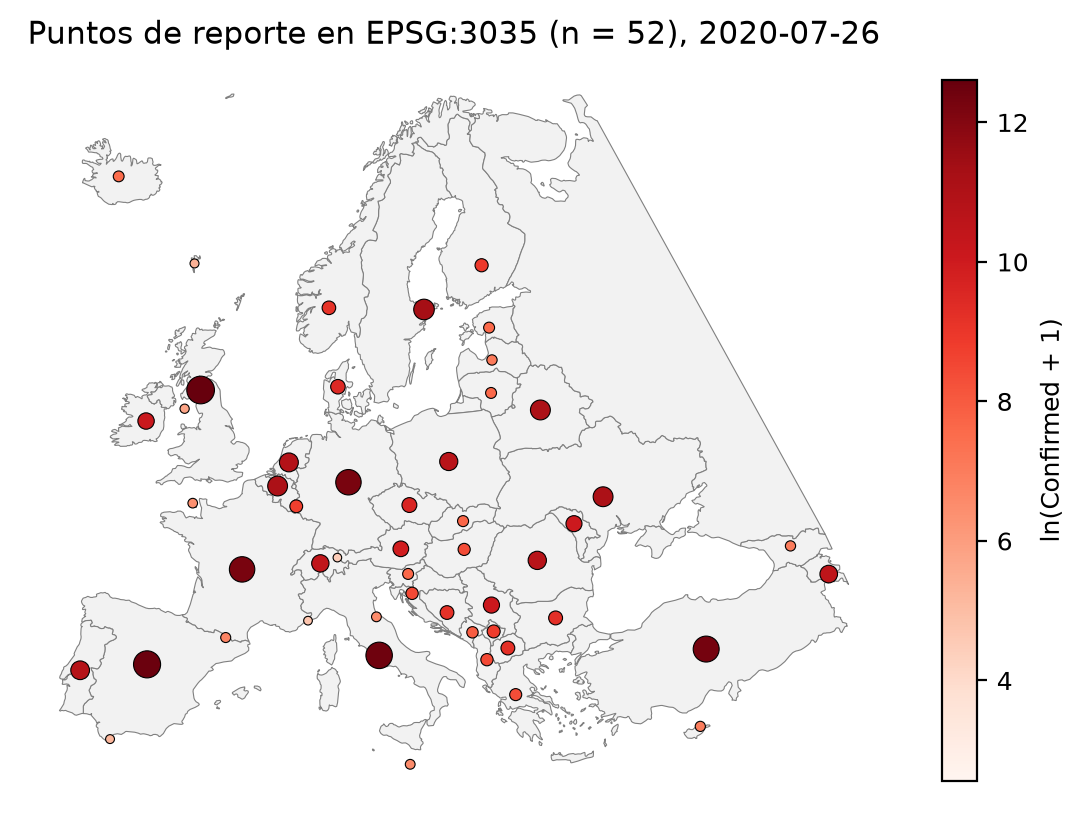
\includegraphics[width=0.55\linewidth]{f1_mapa_puntos.png}
\nota{$n=52$. El color y el tamaño de cada punto representan $\lnC$. Elaboración propia a partir de \citet{dong2020} y \citet{naturalearth}.}
\end{figure}

\subsection{Corte Temporal}

El conjunto de datos constituye un proceso espacio-temporal $Z(s,t)$ en el que cada ubicación se observa en 188 fechas, mientras que la geoestadística clásica supone una única realización de un campo aleatorio $Z(s)$. La combinación de fechas tendría tres consecuencias. Primero, cada sitio aparecería repetido con valores distintos a distancia cero, lo que generaría un efecto pepita espurio y volvería singular la matriz del sistema de Kriging. Segundo, al tratarse de una variable acumulada con tendencia temporal creciente, la variabilidad entre fechas dominaría a la variabilidad espacial, de modo que $\hat\gamma(h)$ reflejaría el crecimiento epidémico y no la dependencia espacial. Tercero, se vulneraría la estacionariedad, puesto que la media y la varianza del proceso cambian con $t$.

La fijación de una fecha $t_0$ produce una sección transversal coherente $Z(s,t_0)$. Se eligió el 26 de julio de 2020, última fecha disponible, porque maximiza la información acumulada, corresponde a un momento posterior al pico de la primera ola en todos los países (Figura~\ref{fig:serie}) y presenta reportes más estables. La alternativa formal, un modelo espacio-temporal con estructura de covarianza separable o no separable \citep{cressie2011}, excede el alcance del presente estudio.

\begin{figure}[H]
\caption{Evolución Acumulada de Casos, Defunciones y Recuperados en la Región Europa de la OMS}\label{fig:serie}
\centering
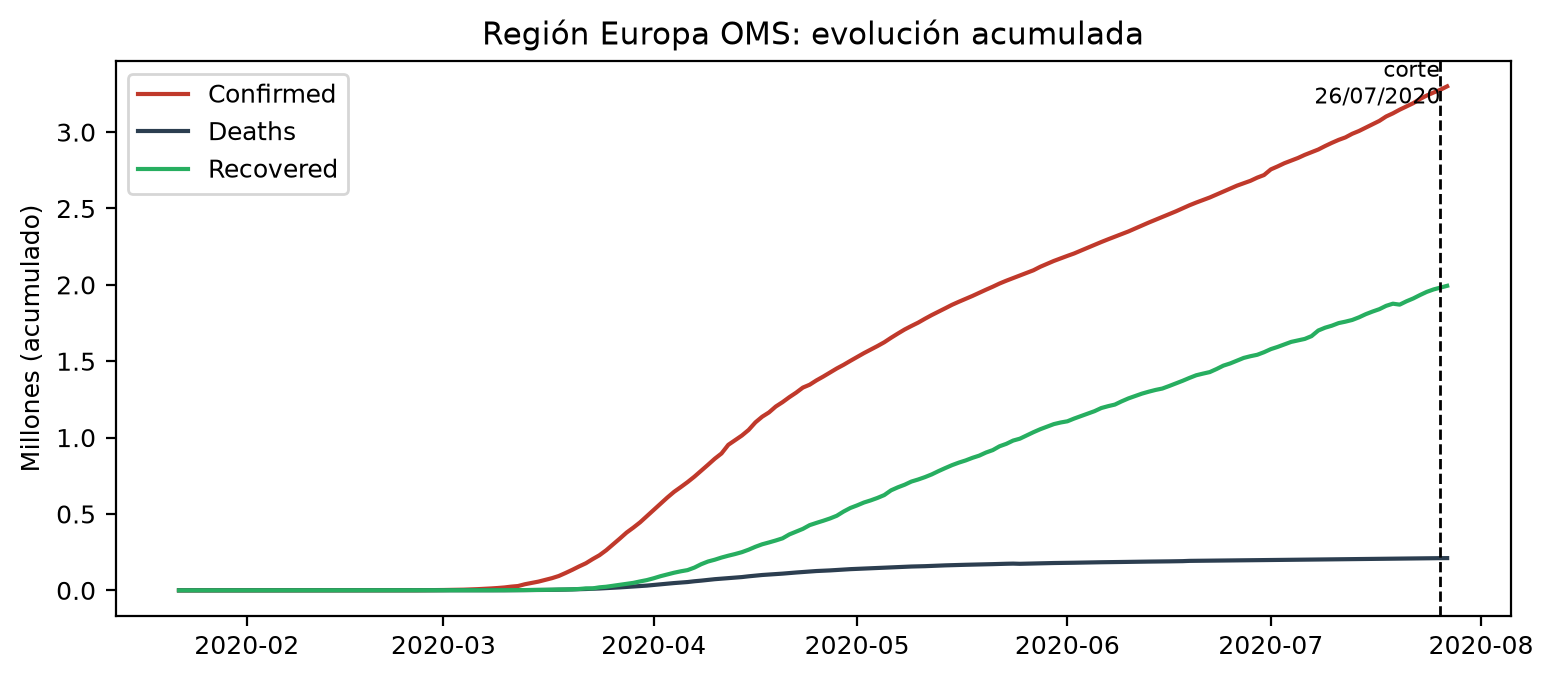
\includegraphics[width=0.8\linewidth]{f1_serie_temporal_europa.png}
\nota{La línea vertical señala la fecha de corte. El 22 de enero de 2020 solo 29 de las 261 ubicaciones del conjunto registraban casos. Elaboración propia a partir de \citet{dong2020}.}
\end{figure}

\subsection{Transformación Logarítmica de los Casos Confirmados}

El semivariograma $\gamma(h)=\tfrac12\mathbb E[(Z(s+h)-Z(s))^2]$ es un momento de segundo orden. Cuando la distribución presenta una cola derecha pesada, unos pocos valores extremos dominan las diferencias al cuadrado: en el área de estudio, cinco países superaban los 200\,000 casos frente a microestados con decenas. El estimador de Matheron carece de robustez ante esta situación, por lo que $\hat\gamma(h)$ se torna errático y refleja la presencia de valores atípicos en lugar de la estructura espacial \citep{cressie1993}. Adicionalmente, el Kriging es el mejor predictor lineal insesgado y solo coincide con la esperanza condicional, óptima en sentido amplio, cuando el campo aleatorio es gaussiano.

Desde el punto de vista metodológico, el crecimiento epidémico es de naturaleza multiplicativa, $C(t)\approx C_0e^{rt}$; en escala logarítmica las diferencias $\ln C_i-\ln C_j=\ln(C_i/C_j)$ expresan razones, más comparables entre países de distinto tamaño, y la transformación estabiliza la varianza. La adición de una unidad evita la indeterminación de $\ln 0$. El modelo resultante corresponde a un Kriging lognormal, cuya predicción se devuelve a la escala original mediante la corrección de sesgo $\hat C(s_0)=\exp\{\hat Z(s_0)+\tfrac12\sigma_K^2(s_0)\}-1$, dado que $\exp(\mathbb E[Z])\neq\mathbb E[\exp Z]$ \citep{journel1980}.

La evidencia empírica respalda la transformación (Tabla~\ref{tab:forma} y Figura~\ref{fig:log}): la asimetría de Confirmed descendió de 2,21 a $-0{,}39$ y la prueba de Shapiro-Wilk dejó de rechazar la normalidad ($p=0{,}357$). Como variable secundaria se eligió Deaths en lugar de Recovered, debido a que esta última registra valor cero en el Reino Unido, los Países Bajos, Suecia y Serbia pese a superar los 1000 casos; dichos ceros obedecen a la ausencia de reporte y no a un fenómeno epidemiológico, por lo que introducirían ceros estructurales en el semivariograma cruzado. La correlación entre $\lnC$ y $\lnD$ en los sitios observados fue $\rho=0{,}957$.

\begin{table}[H]\centering\setstretch{1}\small
\caption{Estadísticos de Forma de las Variables Antes y Después de la Transformación}\label{tab:forma}
\begin{tabular}{lrrrrrr}\toprule
Variable & $M$ & $Mdn$ & $DE$ & Asimetría & Curtosis & Shapiro-Wilk $p$\\\midrule
Confirmed & 42\,659 & 8\,255 & 76\,786 & 2,213 & 3,614 & $<$0,001\\
$\lnC$ & 8,864 & 9,013 & 2,317 & $-0{,}390$ & $-0{,}278$ & 0,357\\
Deaths & 3\,741 & 305 & 9\,514 & 3,151 & 9,063 & $<$0,001\\
$\lnD$ & 5,534 & 5,719 & 2,721 & $-0{,}123$ & $-0{,}420$ & 0,521\\\bottomrule
\end{tabular}
\nota{$n=52$. $M$ = media; $Mdn$ = mediana; $DE$ = desviación estándar. La curtosis se reporta como exceso respecto de la distribución normal. Elaboración propia a partir de \citet{dong2020}.}
\end{table}

\begin{figure}[H]
\caption{Distribución de los Casos Confirmados en Escala Original y Logarítmica}\label{fig:log}
\centering
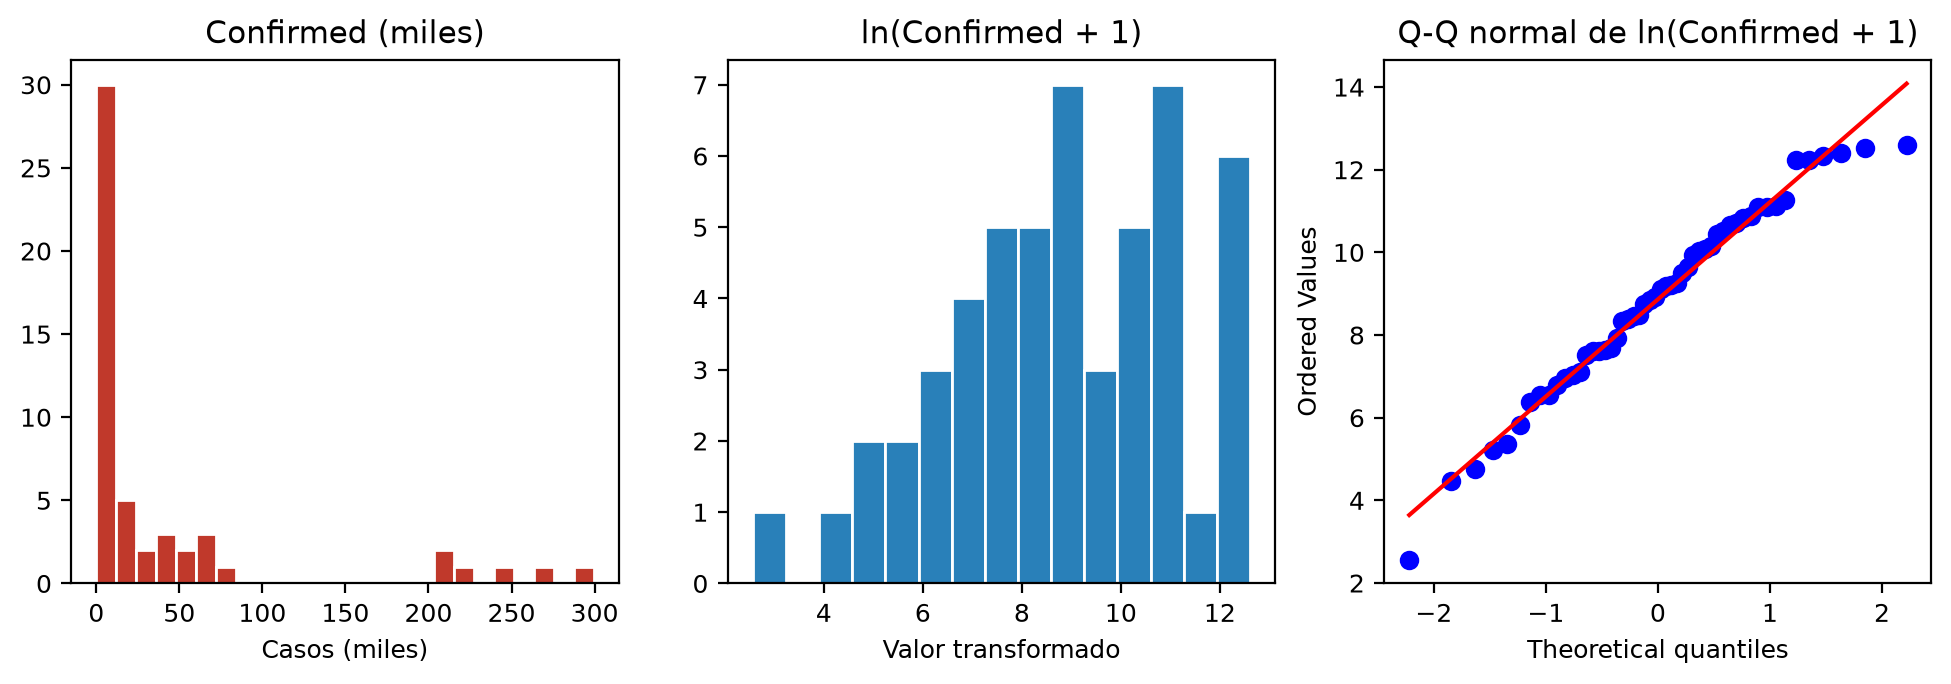
\includegraphics[width=0.95\linewidth]{f1_transformacion_log.png}
\nota{De izquierda a derecha: histograma de Confirmed (miles), histograma de $\lnC$ y gráfico cuantil-cuantil normal de $\lnC$. Elaboración propia.}
\end{figure}

\subsection{Homogeneización del Soporte Espacial}

En geoestadística la variable regionalizada debe referirse a un soporte comparable entre observaciones \citep{gotway2002}. En el presente caso cada dato corresponde al agregado de un país completo, de modo que coexisten unidades como Alemania, con 83 millones de habitantes, y el Estado de la Ciudad del Vaticano, con 808, situado a pocos kilómetros del centroide de Italia. Los pares de observaciones muy próximas con diferencias muy grandes no reflejan una discontinuidad epidemiológica sino una diferencia de soporte, y se manifiestan como un efecto pepita espurio, expresión del problema de la unidad de área modificable \citep{openshaw1984}.

Por esta razón, el análisis de patrones puntuales se realizó con los 52 sitios, dado que su objeto es la localización de los puntos de reporte, mientras que la modelación geoestadística se restringió a las 42 ubicaciones con población igual o superior a 500\,000 habitantes. Quedaron excluidos Andorra, las Islas Feroe, el Vaticano, Islandia, Liechtenstein, Mónaco, San Marino, las Islas del Canal, Gibraltar y la Isla de Man. La Tabla~\ref{tab:soporte} muestra que la homogeneización del soporte redujo la proporción pepita/meseta de 61,7\,\% a 23,3\,\% y que la autocorrelación pasó de nula a positiva. Con la población procedente de Our World in Data se construyó, además, la incidencia acumulada por cada 100\,000 habitantes, empleada en la Fase 4 para separar el riesgo del tamaño poblacional.

\begin{table}[H]\centering\setstretch{1}\small
\caption{Estructura Espacial de $\lnC$ Según el Soporte Considerado}\label{tab:soporte}
\begin{tabular}{lcccc}\toprule
Conjunto & $n$ & Pepita/meseta (\%) & $I$ de Moran & $p$\\\midrule
Todos los sitios & 52 & 61,7 & $-0{,}028$ & 0,498\\
Población $\geq$ 500\,000 & 42 & 23,3 & 0,086 & 0,087\\\bottomrule
\end{tabular}
\nota{La proporción pepita/meseta procede de un modelo exponencial ajustado por mínimos cuadrados ponderados. El índice de Moran emplea una matriz de cinco vecinos más cercanos estandarizada por filas, con valor $p$ obtenido mediante 999 permutaciones. Elaboración propia a partir de \citet{dong2020} y \citet{owid2020}.}
\end{table}

% =====================================================================
\section{Fase 2: Análisis Exploratorio de Datos Espaciales e Interpolación Determinística}
% =====================================================================

\subsection{Estimación de Densidad Kernel y Ancho de Banda}

Sea $\{s_1,\dots,s_n\}$ un patrón puntual observado en la ventana $W\subset\mathbb R^2$. El estimador kernel de la función de intensidad $\lambda(s)$ es \citep{diggle1985,silverman1986}
\[
\hat\lambda_h(s)=\frac{1}{e_h(s)}\sum_{i=1}^{n}\frac{w_i}{h^2}\,K\!\left(\frac{\lVert s-s_i\rVert}{h}\right),\qquad K(u)=\frac{1}{2\pi}e^{-u^2/2},
\]
donde $K$ es un kernel simétrico que integra uno, $h$ es el ancho de banda, $w_i$ es un peso ($w_i=1$ para la intensidad de sitios y $w_i=\text{Confirmed}_i$ para la intensidad de casos) y $e_h(s)$ es una corrección de borde, que en este estudio se fijó en uno porque su efecto se limita a la franja costera.

El ancho de banda gobierna el compromiso entre sesgo y varianza del estimador. Un valor de $h$ pequeño produce una superficie rugosa, con un máximo por cada punto, que permite detectar focos locales pero incorpora artefactos asociados a la posición de los centroides. Un valor grande produce una superficie suave que fusiona focos vecinos en una única mancha regional y diluye los focos reales. Como referencia se empleó la regla de Silverman en dos dimensiones, $h_{opt}=\sigma\,n^{-1/6}$ con $\sigma=\sqrt{(\sigma_x^2+\sigma_y^2)/2}$, y se compararon los anchos $h_{opt}/2$, $h_{opt}$ y $2h_{opt}$ (Figura~\ref{fig:kde} y Tabla~\ref{tab:kde}).

\begin{figure}[H]
\caption{Estimación de Densidad Kernel de Sitios y de Casos Confirmados para Tres Anchos de Banda}\label{fig:kde}
\centering
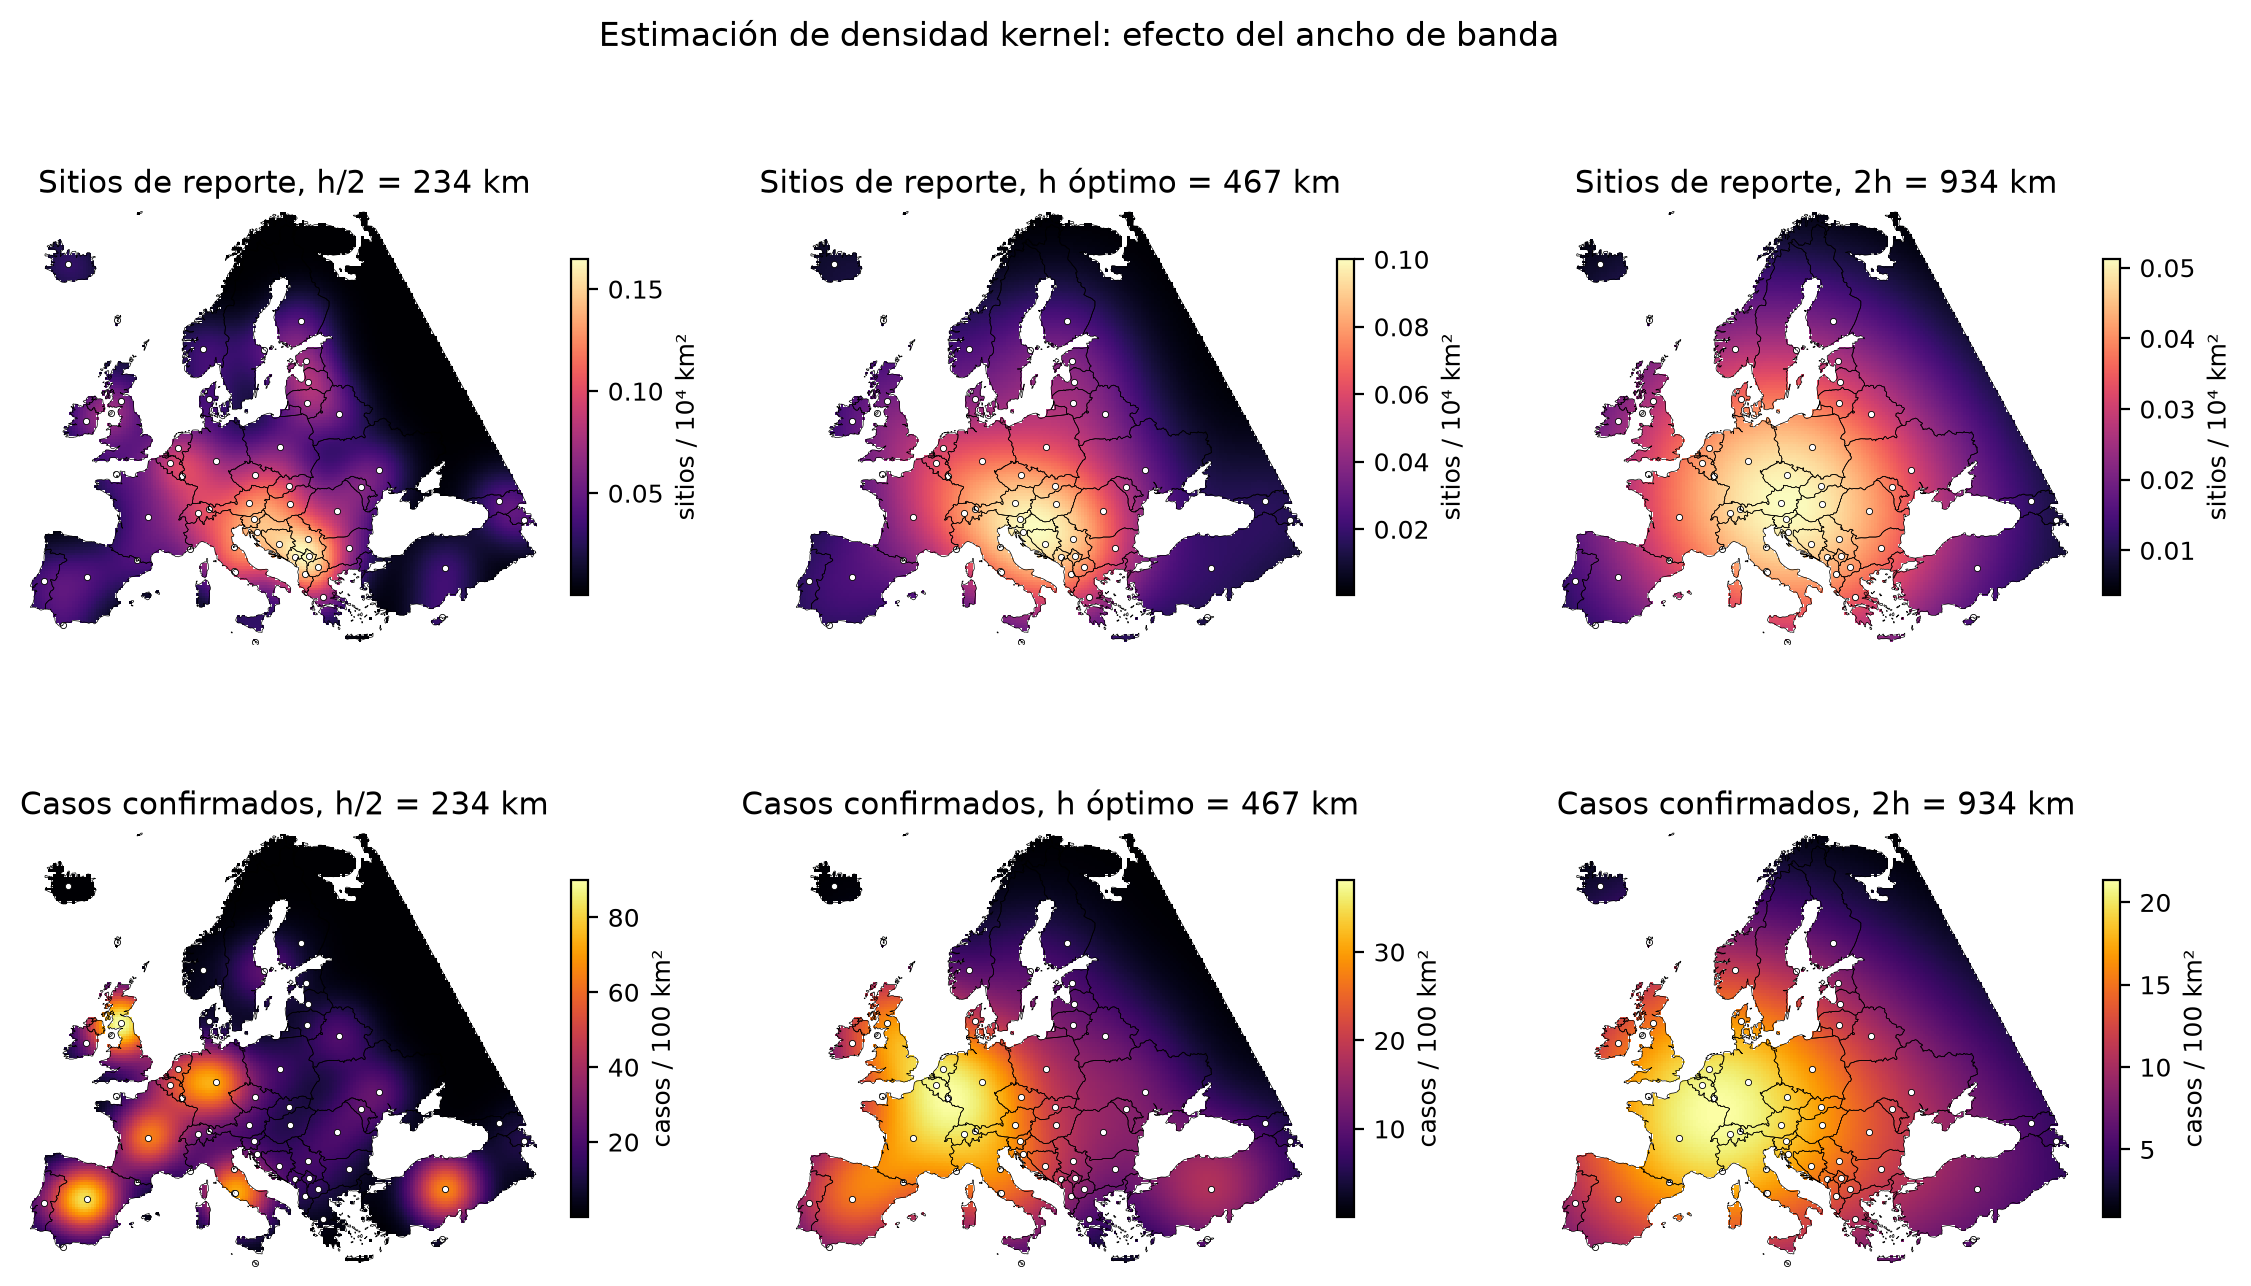
\includegraphics[width=\linewidth]{f2_kde_anchos_banda.png}
\nota{La fila superior representa la intensidad de sitios de reporte y la inferior la intensidad de casos confirmados. $h_{opt}=467$\,km según la regla de Silverman. Elaboración propia.}
\end{figure}

\begin{table}[H]\centering\setstretch{1}\small
\caption{Sensibilidad de la Superficie de Intensidad de Casos al Ancho de Banda}\label{tab:kde}
\begin{tabular}{lcccc}\toprule
Ancho & $h$ (km) & Máximo (casos/100 km²) & Área $>$ 50\,\% del máximo (km²) & $CV$\\\midrule
$h_{opt}/2$ & 234 & 89,9 & 1\,094\,375 & 1,10\\
$h_{opt}$ & 467 & 38,1 & 2\,577\,500 & 0,77\\
$2h_{opt}$ & 934 & 21,4 & 4\,219\,375 & 0,54\\\bottomrule
\end{tabular}
\nota{$CV$ = coeficiente de variación de la superficie estimada sobre la grilla de 25\,km. Elaboración propia.}
\end{table}

Al cuadruplicar el ancho de banda, la intensidad máxima se redujo a la cuarta parte, el área de alta intensidad se cuadruplicó y el coeficiente de variación disminuyó a la mitad. Con $h_{opt}/2$ cada país aparece como un foco aislado y los microestados generan máximos de intensidad de sitios sin significado epidemiológico. Con $h_{opt}$ se identifica un corredor de concentración de casos en Europa occidental que comprende el Reino Unido, Francia, el Benelux, Alemania, España e Italia, y con $2h_{opt}$ dicho corredor se funde en una sola mancha continental. El ancho de banda determina, en consecuencia, la escala, nacional o regional, a la que se identifican los focos, por lo que en vigilancia epidemiológica resulta recomendable reportar al menos dos escalas.

\subsection{Contraste de Completa Aleatoriedad Espacial}

La hipótesis nula de Completa Aleatoriedad Espacial (CSR) establece que los sitios constituyen una realización de un proceso de Poisson homogéneo en $W$, con intensidad constante $\lambda$ e independencia entre puntos; la hipótesis alternativa corresponde a un patrón agregado o regular. La función de distribución de la distancia al vecino más cercano, $G(r)=P(D\le r)$, toma bajo CSR la forma $G(r)=1-e^{-\lambda\pi r^2}$, de modo que $\hat G(r)>G_{CSR}(r)$ en distancias cortas indica agregación. La función $K$ de \citet{ripley1976} se define de manera que $\lambda K(r)$ es el número esperado de puntos adicionales a una distancia no mayor que $r$ de un punto típico, y se estima mediante
\[
\hat K(r)=\frac{|W|}{n(n-1)}\sum_{i\neq j}\mathbb 1(d_{ij}\le r).
\]
Bajo CSR se cumple $K(r)=\pi r^2$. Se empleó la transformación estabilizadora de la varianza $L(r)=\sqrt{K(r)/\pi}$, para la cual $L(r)-r>0$ indica agregación y $L(r)-r<0$ regularidad. Como complemento se consideraron la función de espacio vacío $F(r)$, distribución de la distancia desde un punto arbitrario de $W$ al sitio más cercano, la función $J(r)=(1-G(r))/(1-F(r))$, que vale uno bajo CSR, es menor que uno en patrones agregados y mayor que uno en patrones regulares \citep{vanlieshout1996}, y el índice de \citet{clark1954}, $R=\bar d_{obs}/(0{,}5/\sqrt\lambda)$.

La inferencia se realizó mediante simulación de Monte Carlo \citep{diggle2013,baddeley2015}. Se generaron $m=199$ patrones CSR con el mismo número de puntos dentro de la misma ventana $W$, definida por el territorio continental, lo que compensa los efectos de borde. Para cada función se construyeron envolventes puntuales a partir de los valores mínimo y máximo simulados y, para el contraste global, se utilizó el estadístico de máxima desviación absoluta $T=\max_r|\hat L(r)-\bar L_{CSR}(r)|$, con valor $p=(1+\#\{T_k\ge T_{obs}\})/(m+1)$.

\begin{figure}[H]
\caption{Funciones $G$, $F$, $J$ y $L(r)-r$ Observadas y Envolventes Bajo Completa Aleatoriedad Espacial}\label{fig:csr}
\centering
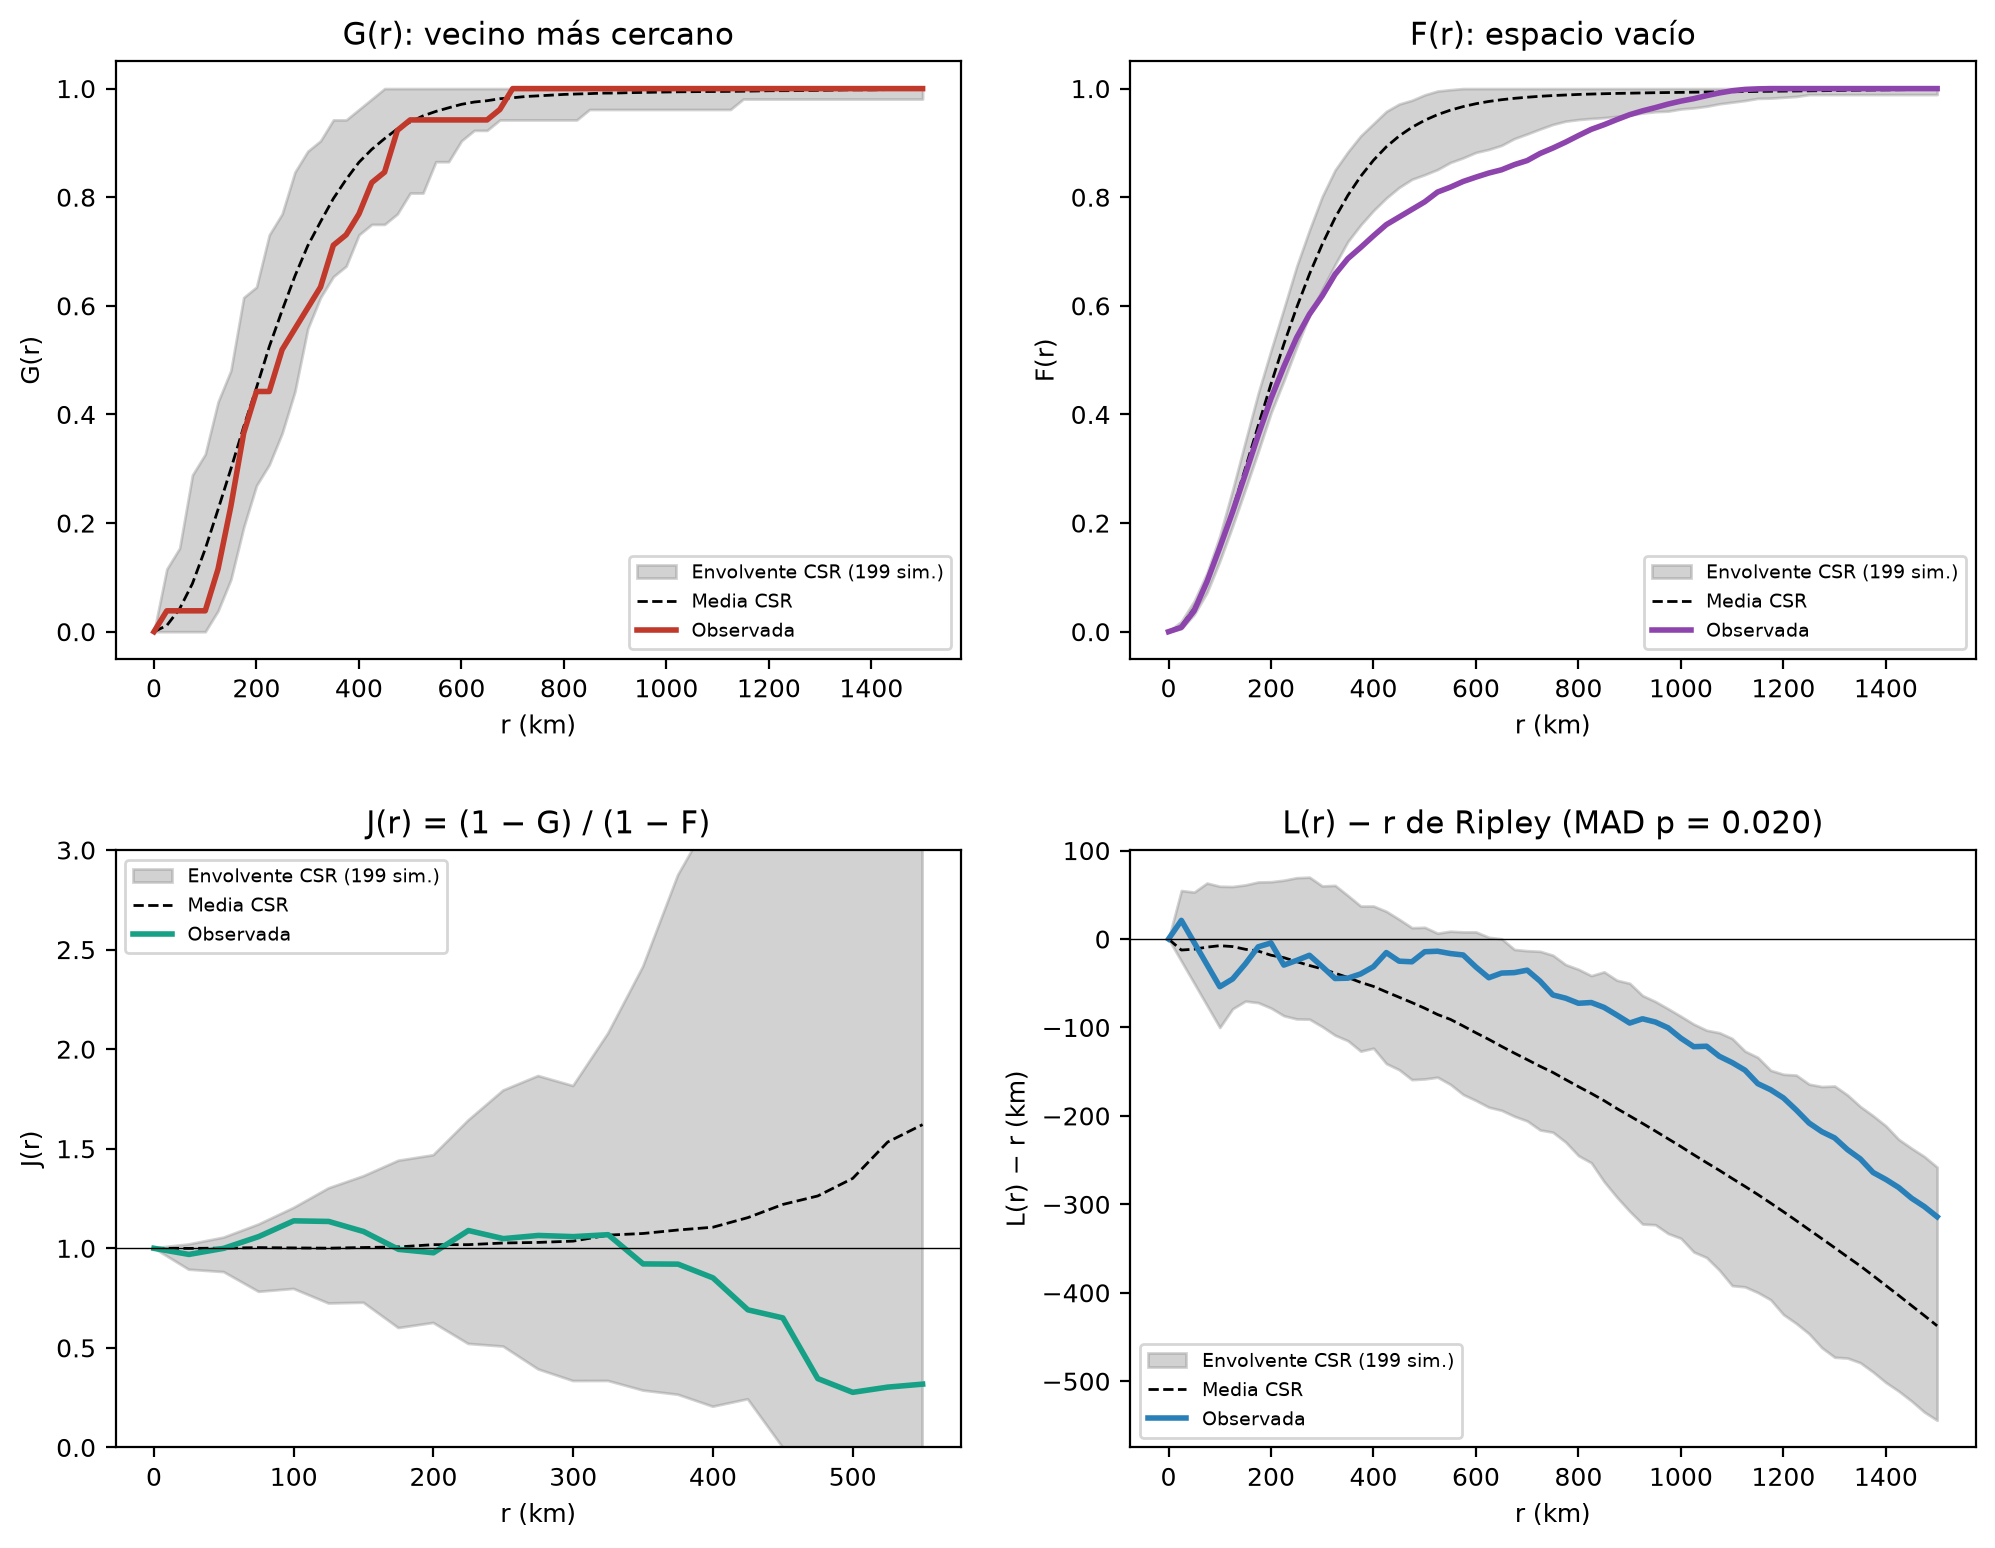
\includegraphics[width=0.88\linewidth]{f2_csr_G_F_J_L.png}
\nota{$n=52$. Las bandas grises corresponden a las envolventes de 199 simulaciones de un proceso de Poisson homogéneo en la misma ventana; la línea discontinua es la media simulada. Elaboración propia.}
\end{figure}

\begin{table}[H]\centering\setstretch{1}\small
\caption{Estadísticos del Patrón de Sitios de Reporte}\label{tab:csr}
\begin{tabular}{lc}\toprule
Estadístico & Valor\\\midrule
Intensidad $\hat\lambda$ (sitios por $10^6$ km²) & 5,875\\
Distancia media al vecino más cercano (km) & 278,1\\
Índice de Clark-Evans $R$ & 1,348\\
Estadístico $z$ de Clark-Evans ($p$ bilateral) & 4,80 ($<$0,001)\\
Estadístico MAD $T_{obs}$ sobre $L(r)$, en km ($p$ de Monte Carlo) & 131,6 (0,020)\\\bottomrule
\end{tabular}
\nota{$n=52$; $|W|=8{,}85\times10^6$ km². MAD = máxima desviación absoluta. Elaboración propia.}
\end{table}

Se rechazó la hipótesis de CSR, con un comportamiento que depende de la escala (Figura~\ref{fig:csr} y Tabla~\ref{tab:csr}). En escalas cortas el patrón es regular: el índice de Clark-Evans fue $R=1{,}35$ ($p<0{,}001$), la distancia al vecino más cercano superó la esperada bajo CSR, $\hat G(r)$ se situó por debajo de la media simulada entre 100 y 450\,km y $\hat J(r)$ fue ligeramente superior a uno. Este comportamiento corresponde a un proceso de inhibición, coherente con la existencia de un único centroide por país. En escalas largas el patrón es agregado: $\hat F(r)$ se situó por debajo de la envolvente entre aproximadamente 400 y 1000\,km, lo que revela amplios espacios vacíos en la Rusia europea, el norte de Escandinavia y Anatolia; $\hat J(r)$ fue inferior a uno a partir de 350\,km y $\hat L(r)-r$ superó la media simulada desde 600\,km. El contraste global confirmó la desviación respecto de CSR ($p=0{,}020$).

Dado que la configuración de los sitios responde a la división político-administrativa y no a la dinámica epidémica, los sitios se trataron como un diseño muestral fijo y el estudio epidemiológico se centró en el atributo observado mediante métodos geoestadísticos. La concentración de sitios en Europa occidental anticipa, además, una mayor incertidumbre de predicción en el este, situación conocida como muestreo preferencial \citep{diggle2010}.

\subsection{Autocorrelación Espacial del Atributo}

Para contrastar la primera ley de la geografía de \citet{tobler1970} sobre el atributo, se calcularon el índice global de \citet{moran1950}, los indicadores locales de asociación espacial \citep[LISA;][]{anselin1995} y el estadístico $G_i^*$ de \citet{getis1992} sobre las 42 ubicaciones del conjunto geoestadístico, con una matriz de cinco vecinos más cercanos estandarizada por filas e inferencia basada en 999 permutaciones (Tabla~\ref{tab:moran} y Figura~\ref{fig:lisa}).

\begin{table}[H]\centering\setstretch{1}\small
\caption{Índice Global de Moran para las Variables Transformadas}\label{tab:moran}
\begin{tabular}{lcccc}\toprule
Variable & $I$ & $E[I]$ & $z$ & $p$\\\midrule
$\lnC$ & 0,086 & $-0{,}024$ & 1,28 & 0,113\\
$\lnD$ & 0,139 & $-0{,}024$ & 1,90 & 0,050\\
$\ln$(incidencia por 100\,000 hab.) & 0,108 & $-0{,}024$ & 1,53 & 0,078\\\bottomrule
\end{tabular}
\nota{$n=42$. Matriz de cinco vecinos más cercanos estandarizada por filas; valores $p$ obtenidos mediante 999 permutaciones. Elaboración propia.}
\end{table}

\begin{figure}[H]
\caption{Indicadores Locales LISA y Estadístico $G_i^*$ de Getis-Ord para la Incidencia Acumulada}\label{fig:lisa}
\centering
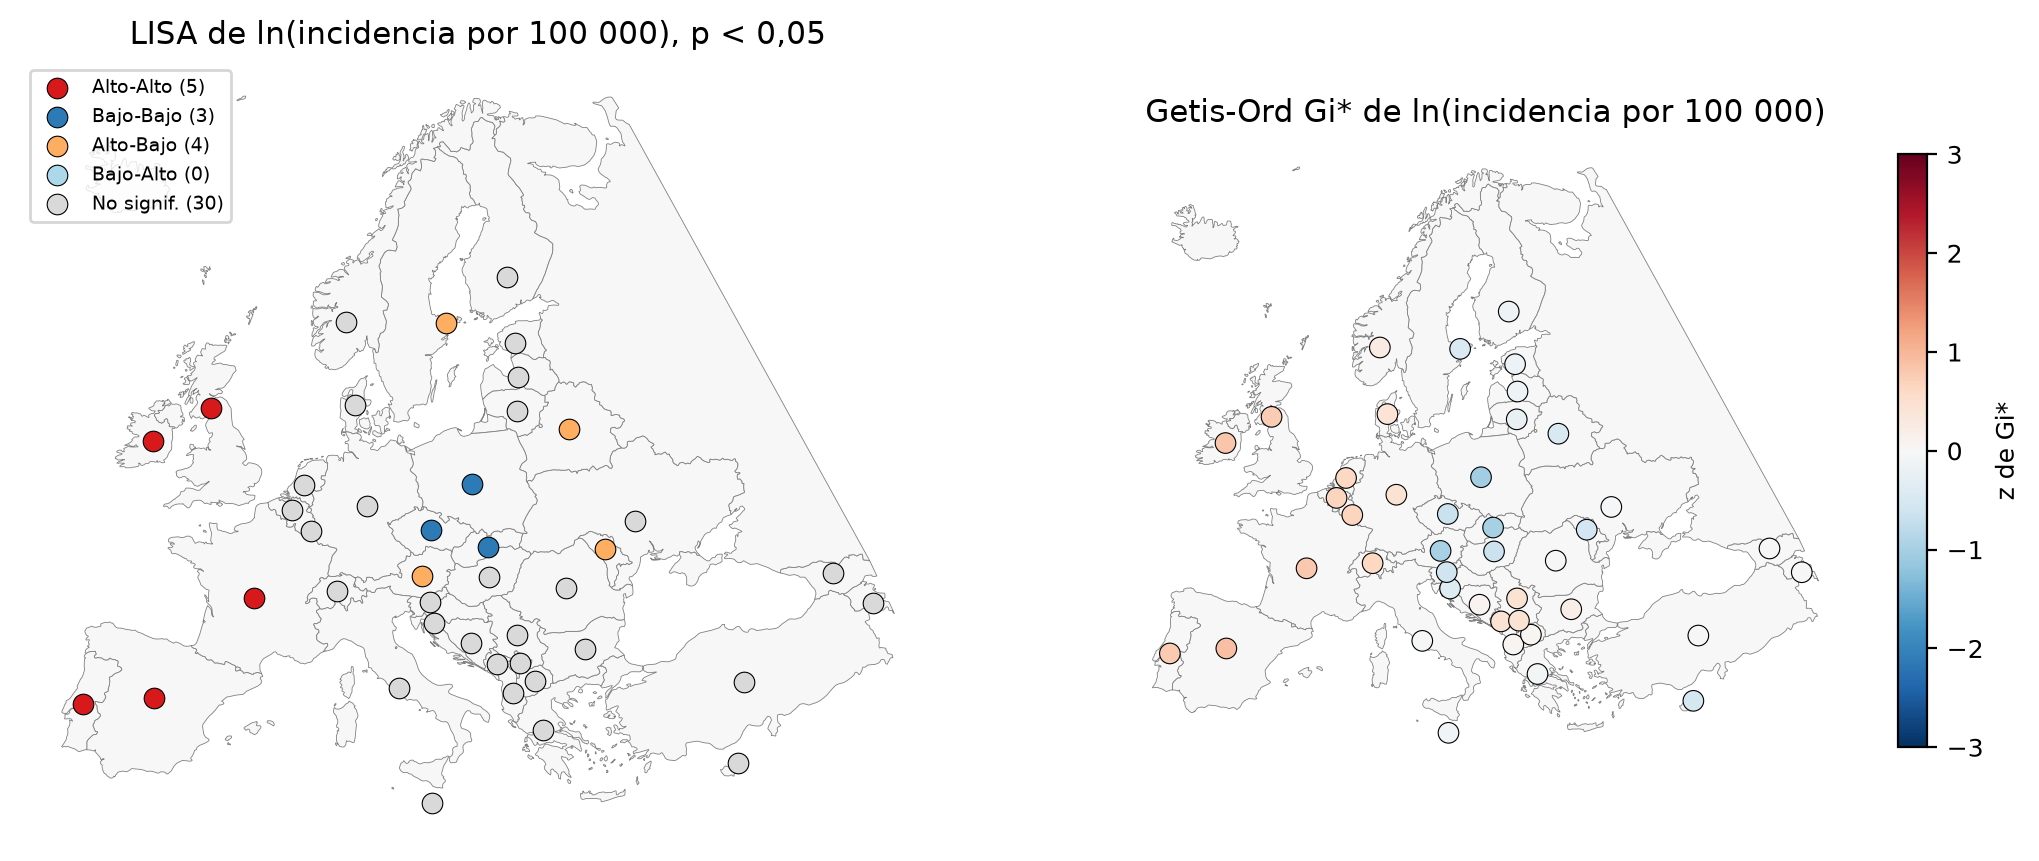
\includegraphics[width=0.9\linewidth]{f2_lisa_getis.png}
\nota{Panel izquierdo: clasificación LISA con $p<0{,}05$. Panel derecho: valor $z$ del estadístico $G_i^*$. Incidencia expresada en casos por 100\,000 habitantes. Elaboración propia a partir de \citet{dong2020} y \citet{owid2020}.}
\end{figure}

La autocorrelación global resultó positiva y de magnitud moderada, lo que es esperable con 42 observaciones; solo la correspondiente a las defunciones alcanzó el umbral convencional de significación ($p=0{,}050$). En el nivel local los patrones son nítidos. Se identificó un conglomerado Alto-Alto en el litoral atlántico occidental, integrado por España, Portugal, Francia, el Reino Unido e Irlanda, y un conglomerado Bajo-Bajo en Europa central, formado por Polonia, Eslovaquia y Chequia. Suecia, Bielorrusia, Moldavia y Austria se clasificaron como valores atípicos Alto-Bajo; en los tres primeros casos, la clasificación es consistente con estrategias de contención menos restrictivas que las de sus vecinos. Estos resultados indican que la heterogeneidad espacial obedece tanto a la distancia como a decisiones nacionales de política sanitaria.

\subsection{Formulación del Interpolador por Inverso de la Distancia}

Para una localización no muestreada $s_0$ y $Z(s_i)=\ln(\text{Confirmed}_i+1)$, el interpolador ponderado por el inverso de la distancia \citep{shepard1968} es
\[
\hat Z_{IDW}(s_0)=\sum_{i=1}^{n}\lambda_i(s_0)\,Z(s_i),\qquad
\lambda_i(s_0)=\frac{d(s_0,s_i)^{-p}}{\sum_{k=1}^{n}d(s_0,s_k)^{-p}},\qquad p>0,
\]
donde $d$ es la distancia euclidiana en el plano proyectado, expresada en kilómetros. Los pesos son positivos y suman uno, de modo que $\hat Z(s_0)$ queda acotado entre el mínimo y el máximo observados. Si $s_0$ coincide con un sitio muestreado, $\hat Z(s_0)=Z(s_i)$, por lo que el método es un interpolador exacto.

\subsection{Efecto del Parámetro de Potencia y Limitaciones del Método}

El parámetro $p$ controla el equilibrio entre suavizado global y fidelidad local. Cuando $p$ tiende a cero, los pesos se igualan y la predicción converge a la media aritmética, lo que produce una superficie plana. Con valores pequeños de $p$ los puntos lejanos conservan influencia y la superficie es suave, mientras que con valores grandes domina el vecino más cercano; en el límite $p\to\infty$ la superficie converge a los polígonos de Voronoi y aparecen discontinuidades concéntricas alrededor de cada dato.

Frente a la regresión espacial y al Kriging, el método presenta seis limitaciones \citep{isaaks1989,webster2007}: (a) el parámetro $p$ es arbitrario y no se deriva de la estructura de dependencia de los datos; (b) no proporciona varianza de predicción y, por tanto, no cuantifica la incertidumbre; (c) no corrige la redundancia de los datos agrupados, cuyos pesos se acumulan como si aportaran información independiente, mientras que el Kriging la descuenta mediante la matriz $\Gamma$; (d) es isotrópico y no admite tendencias ni covariables, a diferencia de la regresión espacial y del Kriging Universal; (e) no permite extrapolar fuera del rango observado; y (f) carece de optimalidad estadística, mientras que el Kriging es el mejor predictor lineal insesgado.

\begin{table}[H]\centering\setstretch{1}\small
\caption{Validación Cruzada del Interpolador IDW Según el Parámetro de Potencia}\label{tab:idw}
\begin{tabular}{lcccccccc}\toprule
$p$ & 0,5 & 1 & 1,5 & 2 & 2,5 & 3 & 4 & 6\\\midrule
RMSE & 1,694 & 1,664 & 1,655 & 1,685 & 1,749 & 1,826 & 1,958 & 2,084\\
ME & $-0{,}04$ & $-0{,}10$ & $-0{,}15$ & $-0{,}20$ & $-0{,}24$ & $-0{,}27$ & $-0{,}31$ & $-0{,}37$\\\bottomrule
\end{tabular}
\nota{$n=42$. Validación cruzada dejando uno fuera sobre $\lnC$. RMSE = raíz del error cuadrático medio; ME = error medio. Elaboración propia.}
\end{table}

\begin{figure}[H]
\caption{Selección del Parámetro de Potencia y Superficies Interpoladas por IDW}\label{fig:idw}
\centering
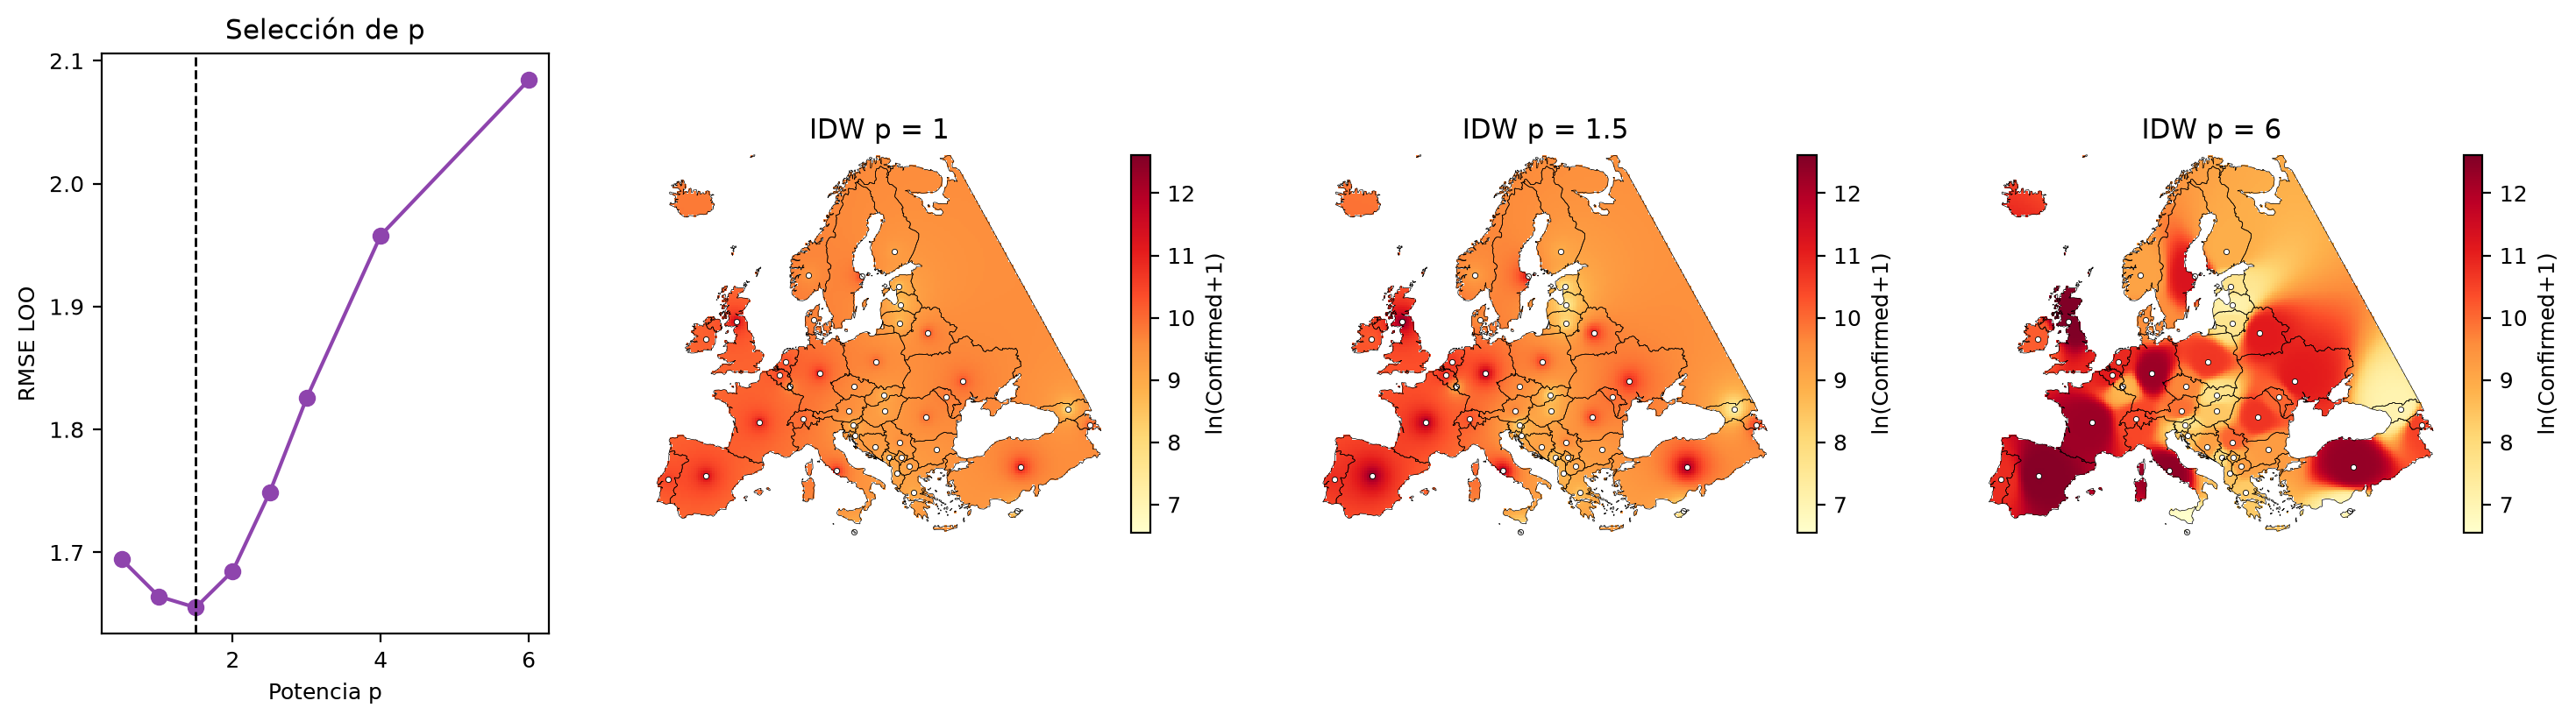
\includegraphics[width=\linewidth]{f2_idw_potencias.png}
\nota{El primer panel muestra el RMSE de validación cruzada en función de $p$; los restantes, las superficies de $\lnC$ con $p=1$, $p=1{,}5$ y $p=6$. Elaboración propia.}
\end{figure}

La validación cruzada seleccionó $p=1{,}5$, con un RMSE de 1,655, valor inferior al obtenido con el parámetro convencional $p=2$ (Tabla~\ref{tab:idw} y Figura~\ref{fig:idw}). Con $p=6$ el RMSE aumentó en 26\,\% y la superficie adoptó la forma de un mosaico de Voronoi. El sesgo medio creció con $p$, debido a que los sitios aislados con valores bajos dominan sus vecindades. Aun con el valor óptimo, el método no informa sobre la confiabilidad de cada predicción, limitación que justifica el enfoque geoestadístico desarrollado a continuación.

% =====================================================================
\section{Fase 3: Modelación Geoestadística Mediante Kriging y Cokriging}
% =====================================================================

Sea $\{Z(s):s\in D\subset\mathbb R^2\}$ una función aleatoria. Bajo estacionariedad de segundo orden, con $E[Z(s)]=\mu$ y $\operatorname{Cov}[Z(s),Z(s+h)]=C(h)$, se cumple
\[
\gamma(h)=\tfrac12 E\big[(Z(s+h)-Z(s))^2\big]=C(0)-C(h),
\]
de modo que la meseta coincide con la varianza $C(0)$. La hipótesis intrínseca, que solo exige la estacionariedad de los incrementos, es más débil y constituye el supuesto requerido por el Kriging Ordinario \citep{matheron1963}.

\subsection{Semivariograma Experimental y Parámetros Estructurales}

El estimador de Matheron del semivariograma de $Z=\lnC$ es
\[
\hat\gamma(h)=\frac{1}{2|N(h)|}\sum_{(i,j)\in N(h)}\big[Z(s_i)-Z(s_j)\big]^2,\qquad N(h)=\{(i,j):\lVert s_i-s_j\rVert\in(h-\delta,\,h+\delta]\},
\]
y se calculó con 12 clases equiespaciadas hasta la mitad de la distancia máxima entre sitios (2241\,km), con entre 11 y 80 pares por clase. Sus parámetros estructurales se definen en la Tabla~\ref{tab:param}. El efecto pepita recoge la variabilidad a escalas inferiores a la distancia mínima entre sitios y el error de medición, atribuibles en este contexto a diferencias en la capacidad diagnóstica, el subregistro y la definición de caso entre países vecinos. La meseta representa la variabilidad total de la carga epidémica entre ubicaciones independientes, y el alcance, la distancia dentro de la cual la carga de un país aporta información sobre la de sus vecinos, asociada a la movilidad transfronteriza y a los corredores de transporte. La razón $c_0/(c_0+c)$ indica una dependencia espacial fuerte cuando es inferior a 25\,\%, moderada entre 25 y 75\,\% y débil cuando supera 75\,\% \citep{cambardella1994}.

\begin{table}[H]\centering\setstretch{1}\small
\caption{Definición y Significado de los Parámetros del Semivariograma}\label{tab:param}
\begin{tabularx}{\linewidth}{>{\raggedright\arraybackslash}p{2.6cm}>{\raggedright\arraybackslash}p{3.6cm}X}\toprule
Parámetro & Definición & Significado físico-epidemiológico\\\midrule
Efecto pepita $c_0$ & $\lim_{h\to0^+}\gamma(h)$ & Variabilidad a microescala y error de medición: diferencias de capacidad diagnóstica, subregistro y definición de caso entre países contiguos\\
Meseta $c_0+c$ & $\lim_{h\to\infty}\gamma(h)=C(0)$ & Variabilidad total de la carga epidémica; $c$ es la fracción con estructura espacial\\
Alcance $a$ & Distancia a la que $\gamma$ alcanza la meseta (95\,\% en modelos asintóticos) & Escala de contagio y movilidad: más allá de $a$ las cargas de dos países son independientes\\\bottomrule
\end{tabularx}
\nota{Elaboración propia a partir de \citet{cressie1993} y \citet{webster2007}.}
\end{table}

\subsection{Modelos Teóricos de Semivariograma}

Con $c_0$ el efecto pepita, $c$ la meseta parcial y $a$ el alcance práctico, los tres modelos considerados se expresan, para $h>0$, como sigue:
\begin{align*}
\text{Esférico: }&\gamma(h)=c_0+c\left[\tfrac32\tfrac{h}{a}-\tfrac12\big(\tfrac{h}{a}\big)^3\right]\ \text{si } h\le a;\quad \gamma(h)=c_0+c\ \text{si } h>a,\\
\text{Exponencial: }&\gamma(h)=c_0+c\left[1-\exp(-3h/a)\right],\\
\text{Gaussiano: }&\gamma(h)=c_0+c\left[1-\exp(-3h^2/a^2)\right].
\end{align*}
Sus propiedades se comparan en la Tabla~\ref{tab:modelos}. Para una variable de transmisión epidémica medida en soporte puntual cabe esperar un comportamiento lineal en el origen, propio de los modelos exponencial y esférico, puesto que el contagio decae con la distancia de forma continua pero no suave, con discontinuidades en las fronteras y eventos de superpropagación. No obstante, cuando los datos son agregados de área, la regularización sobre bloques suaviza el semivariograma en las proximidades del origen y lo aproxima a un comportamiento parabólico, característico del modelo gaussiano \citep{journel1978}. La elección final debe, por tanto, contrastarse con los datos.

\begin{table}[H]\centering\setstretch{1}\small
\caption{Propiedades de los Modelos Teóricos de Semivariograma}\label{tab:modelos}
\begin{tabularx}{\linewidth}{>{\raggedright\arraybackslash}p{3.8cm}XXX}\toprule
Propiedad & Esférico & Exponencial & Gaussiano\\\midrule
Comportamiento en el origen & Lineal & Lineal, con mayor pendiente & Parabólico\\
Regularidad del campo & Continuo, no diferenciable & Continuo, no diferenciable & Diferenciable\\
Meseta & Alcanzada en $a$ & Asintótica & Asintótica\\
Condicionamiento del sistema & Adecuado & Adecuado & Deficiente si $c_0\approx0$\\\bottomrule
\end{tabularx}
\nota{Elaboración propia a partir de \citet{chiles2012} y \citet{journel1978}.}
\end{table}

\subsubsection{Estimación y Selección del Modelo}

Se compararon tres métodos de estimación de los parámetros $\theta=(c_0,c,a)$ \citep{cressie1985,patterson1971,diggle1998}. El método de mínimos cuadrados ponderados de Cressie (WLS) minimiza $\sum_k|N(h_k)|\big[\hat\gamma(h_k)/\gamma(h_k;\theta)-1\big]^2$ y aproxima los mínimos cuadrados generalizados, dado que $\operatorname{Var}[\hat\gamma(h)]\approx2\gamma(h)^2/|N(h)|$. La máxima verosimilitud (MV) supone $\mathbf Z\sim N(\mu\mathbf 1,\Sigma_\theta)$, con $\Sigma_\theta=C(0)\mathbf I-\Gamma_\theta$, y minimiza
\[
-\ell(\theta)=\tfrac12\big[\ln|\Sigma_\theta|+(\mathbf z-\hat\mu\mathbf 1)^\top\Sigma_\theta^{-1}(\mathbf z-\hat\mu\mathbf 1)+n\ln2\pi\big],
\]
con $\hat\mu$ estimado por mínimos cuadrados generalizados. La máxima verosimilitud restringida (REML) corrige el sesgo de la MV en la estimación de la varianza mediante el término adicional $\tfrac12\ln(\mathbf 1^\top\Sigma_\theta^{-1}\mathbf 1)$. El criterio de selección fue el siguiente: entre los ajustes con matriz de Kriging bien condicionada, con número de condición $\kappa(A)<10^6$, y con varianza calibrada, $|\text{RMSS}-1|<0{,}1$, se eligió el de menor RMSE en validación cruzada dejando uno fuera.

\begin{table}[H]\centering\setstretch{1}\small
\caption{Parámetros y Validación Cruzada de los Semivariogramas Ajustados para $\lnC$}\label{tab:vario}
\begin{tabular}{llrrrrcc}\toprule
Método & Modelo & $c_0$ & $c$ & $a$ (km) & $c_0/(c_0+c)$ (\%) & RMSE & RMSS\\\midrule
WLS & Esférico & 1,268 & 2,257 & 2418 & 36,0 & 1,767 & 1,191\\
WLS & Exponencial & 0,196 & 3,196 & 1858 & 5,8 & 1,823 & 1,280\\
WLS & Gaussiano & 1,745 & 1,890 & 2324 & 48,0 & 1,753 & 1,167\\
MV & Esférico & 0,000 & 2,801 & 488 & 0,0 & 1,601 & 1,006\\
MV & Exponencial & 0,000 & 2,880 & 641 & 0,0 & 1,649 & 1,014\\
MV & Gaussiano & 0,000 & 2,899 & 393 & 0,0 & 1,583 & 1,019\\
REML & Esférico & 0,000 & 3,047 & 576 & 0,0 & 1,641 & 1,024\\
REML & Exponencial & 0,000 & 3,070 & 745 & 0,0 & 1,670 & 1,015\\
REML & Gaussiano & 0,000 & 3,002 & 400 & 0,0 & 1,587 & 1,012\\\bottomrule
\end{tabular}
\nota{$n=42$; varianza muestral de $\lnC$ igual a 2,914. RMSE y RMSS proceden de la validación cruzada dejando uno fuera del Kriging Ordinario. WLS = mínimos cuadrados ponderados; MV = máxima verosimilitud; REML = máxima verosimilitud restringida. El modelo seleccionado es el gaussiano estimado por MV. Elaboración propia.}
\end{table}

\begin{figure}[H]
\caption{Semivariograma Experimental de $\lnC$ y Modelos Teóricos Ajustados}\label{fig:vario}
\centering
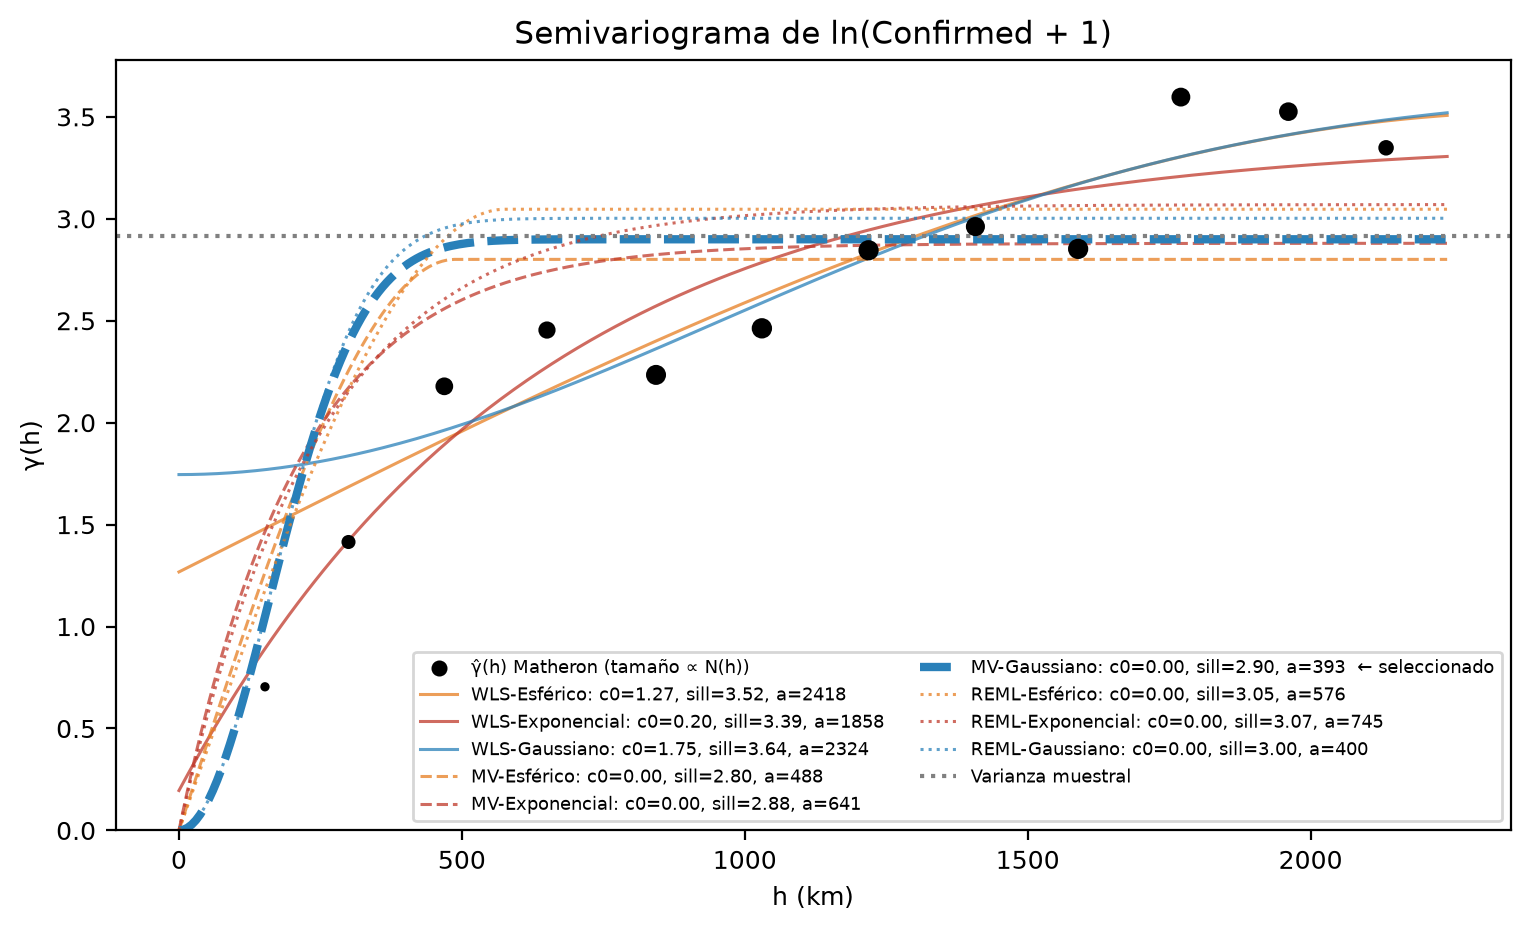
\includegraphics[width=0.8\linewidth]{f3_semivariograma_confirmed.png}
\nota{El tamaño de los puntos es proporcional al número de pares por clase. Líneas continuas: WLS; discontinuas: MV; punteadas: REML. La línea gruesa corresponde al modelo seleccionado. Elaboración propia.}
\end{figure}

Los ajustes por WLS reproducen el semivariograma experimental a gran escala, con alcances entre 1858 y 2418\,km, pero el semivariograma experimental continúa creciendo más allá de 1500\,km, lo que sugiere una variación de gran escala asociada al gradiente oeste-este de la primera ola más que una meseta estacionaria (Tabla~\ref{tab:vario} y Figura~\ref{fig:vario}). Los métodos de verosimilitud, que utilizan la matriz de covarianza completa y no dependen de la agrupación en clases, estimaron un efecto pepita nulo y alcances entre 393 y 745\,km. En validación cruzada, los ajustes por verosimilitud obtuvieron un RMSE entre 1,58 y 1,67 y un RMSS entre 1,01 y 1,02, frente a un RMSE entre 1,75 y 1,82 y un RMSS entre 1,17 y 1,28 en los ajustes por WLS, cuyas varianzas resultaron subestimadas. Este resultado concuerda con la teoría asintótica del Kriging, según la cual la calidad de la interpolación depende principalmente del comportamiento del semivariograma en las proximidades del origen \citep{stein1999}, región que la verosimilitud estima con mayor precisión.

El modelo seleccionado fue el gaussiano estimado por MV, con $c_0\approx0$, $c=2{,}899$ y $a=393$\,km. Su comportamiento parabólico en el origen es consistente con la regularización inherente a los datos agregados por país, y la diferencia frente al modelo esférico estimado por MV fue reducida (RMSE de 1,583 frente a 1,601), lo que indica que las conclusiones son robustas a la elección del modelo. La ausencia de efecto pepita denota una dependencia espacial fuerte una vez homogeneizado el soporte, y el alcance de aproximadamente 390\,km corresponde a la escala de países contiguos: a distancias mayores, la carga epidémica de un país no aporta información sobre la de otro.

\subsection{Sistema del Kriging Ordinario para las Defunciones}

Sea $Z_2(s)=\lnD$, con media constante y desconocida $\mu$, y sea $\hat Z_2(s_0)=\sum_{i=1}^n\lambda_iZ_2(s_i)$ el predictor lineal. La condición de insesgadez $E[\hat Z_2(s_0)-Z_2(s_0)]=\mu\big(\sum_i\lambda_i-1\big)=0$ se cumple para todo $\mu$ si y solo si $\sum_{i=1}^n\lambda_i=1$. Bajo la hipótesis intrínseca y con dicha restricción, la varianza del error de estimación es
\[
\sigma_E^2(s_0)=\operatorname{Var}[\hat Z_2(s_0)-Z_2(s_0)]=2\sum_{i}\lambda_i\gamma(s_i,s_0)-\sum_{i}\sum_{j}\lambda_i\lambda_j\gamma(s_i,s_j).
\]
La minimización de $\sigma_E^2$ sujeta a la restricción, mediante el lagrangiano $\mathcal L=\sigma_E^2+2\mu_L\big(\sum_i\lambda_i-1\big)$, conduce al sistema
\[
\sum_{j=1}^n\lambda_j\gamma(s_i,s_j)+\mu_L=\gamma(s_i,s_0),\quad i=1,\dots,n;\qquad\sum_{j=1}^n\lambda_j=1,
\]
que en forma matricial se escribe
\[
\begin{pmatrix}\gamma_{11}&\cdots&\gamma_{1n}&1\\\vdots&\ddots&\vdots&\vdots\\\gamma_{n1}&\cdots&\gamma_{nn}&1\\1&\cdots&1&0\end{pmatrix}
\begin{pmatrix}\lambda_1\\\vdots\\\lambda_n\\\mu_L\end{pmatrix}=
\begin{pmatrix}\gamma_{10}\\\vdots\\\gamma_{n0}\\1\end{pmatrix},\qquad
\sigma^2_{OK}(s_0)=\sum_{i=1}^n\lambda_i\gamma_{i0}+\mu_L.
\]
Si $\gamma$ es condicionalmente definida negativa, la matriz del sistema es invertible y la solución es única \citep{cressie1993}.

Para $\lnD$ se aplicó el mismo procedimiento de estimación y selección. El modelo elegido fue el esférico estimado por REML, con $c_0=3{,}25$ y un alcance situado en el límite superior de búsqueda, de aproximadamente 8965\,km; el semivariograma no alcanza la meseta dentro del dominio, comportamiento característico de la presencia de una deriva. La regresión de $\lnD$ sobre las coordenadas confirmó un gradiente oeste-este significativo ($p=0{,}003$ para la coordenada $x$; $R^2=0{,}22$), coherente con la mayor mortalidad registrada en Europa occidental durante la primera ola.

En consecuencia, se contrastó el Kriging Ordinario con un Kriging Universal con deriva lineal $m(s)=\beta_0+\beta_1x+\beta_2y$, que incorpora las restricciones $\sum_i\lambda_if_k(s_i)=f_k(s_0)$:
\[
\begin{pmatrix}\Gamma&\mathbf F\\\mathbf F^\top&\mathbf 0\end{pmatrix}\begin{pmatrix}\bm\lambda\\\bm\mu\end{pmatrix}=\begin{pmatrix}\bm\gamma_0\\\mathbf f_0\end{pmatrix},\qquad\mathbf F=[\mathbf 1,\mathbf x,\mathbf y],
\]
con $\Gamma$ estimado sobre los residuos de la deriva. El Kriging Universal no mejoró la predicción (Tabla~\ref{tab:deaths}): obtuvo un RMSE entre 2,24 y 2,31 y un RMSS entre 1,23 y 1,28, frente a 2,06 y 1,01 del Kriging Ordinario. Este último reestima la media en cada vecindad y absorbe la deriva sin el costo de estimar $\bm\beta$ con 42 observaciones, por lo que se adoptó para la cartografía de las defunciones (Figura~\ref{fig:okdeaths}).

\begin{table}[H]\centering\setstretch{1}\small
\caption{Validación Cruzada del Kriging Ordinario y del Kriging Universal para $\lnD$}\label{tab:deaths}
\begin{tabular}{lccccc}\toprule
Estimador & ME & MAE & RMSE & $r$ & RMSS\\\midrule
Kriging Ordinario (esférico, REML) & 0,004 & 1,675 & 2,058 & 0,303 & 1,014\\
Kriging Universal (esférico) & $-0{,}040$ & 1,878 & 2,307 & 0,188 & 1,270\\
Kriging Universal (exponencial) & $-0{,}017$ & 1,809 & 2,243 & 0,230 & 1,232\\
Kriging Universal (gaussiano) & $-0{,}039$ & 1,892 & 2,308 & 0,186 & 1,276\\\bottomrule
\end{tabular}
\nota{$n=42$. Validación cruzada dejando uno fuera. ME = error medio; MAE = error absoluto medio; $r$ = correlación entre valores observados y predichos; RMSS = raíz del error cuadrático medio estandarizado. Elaboración propia.}
\end{table}

\begin{figure}[H]
\caption{Predicción por Kriging Ordinario de $\lnD$ y Desviación Estándar del Error}\label{fig:okdeaths}
\centering
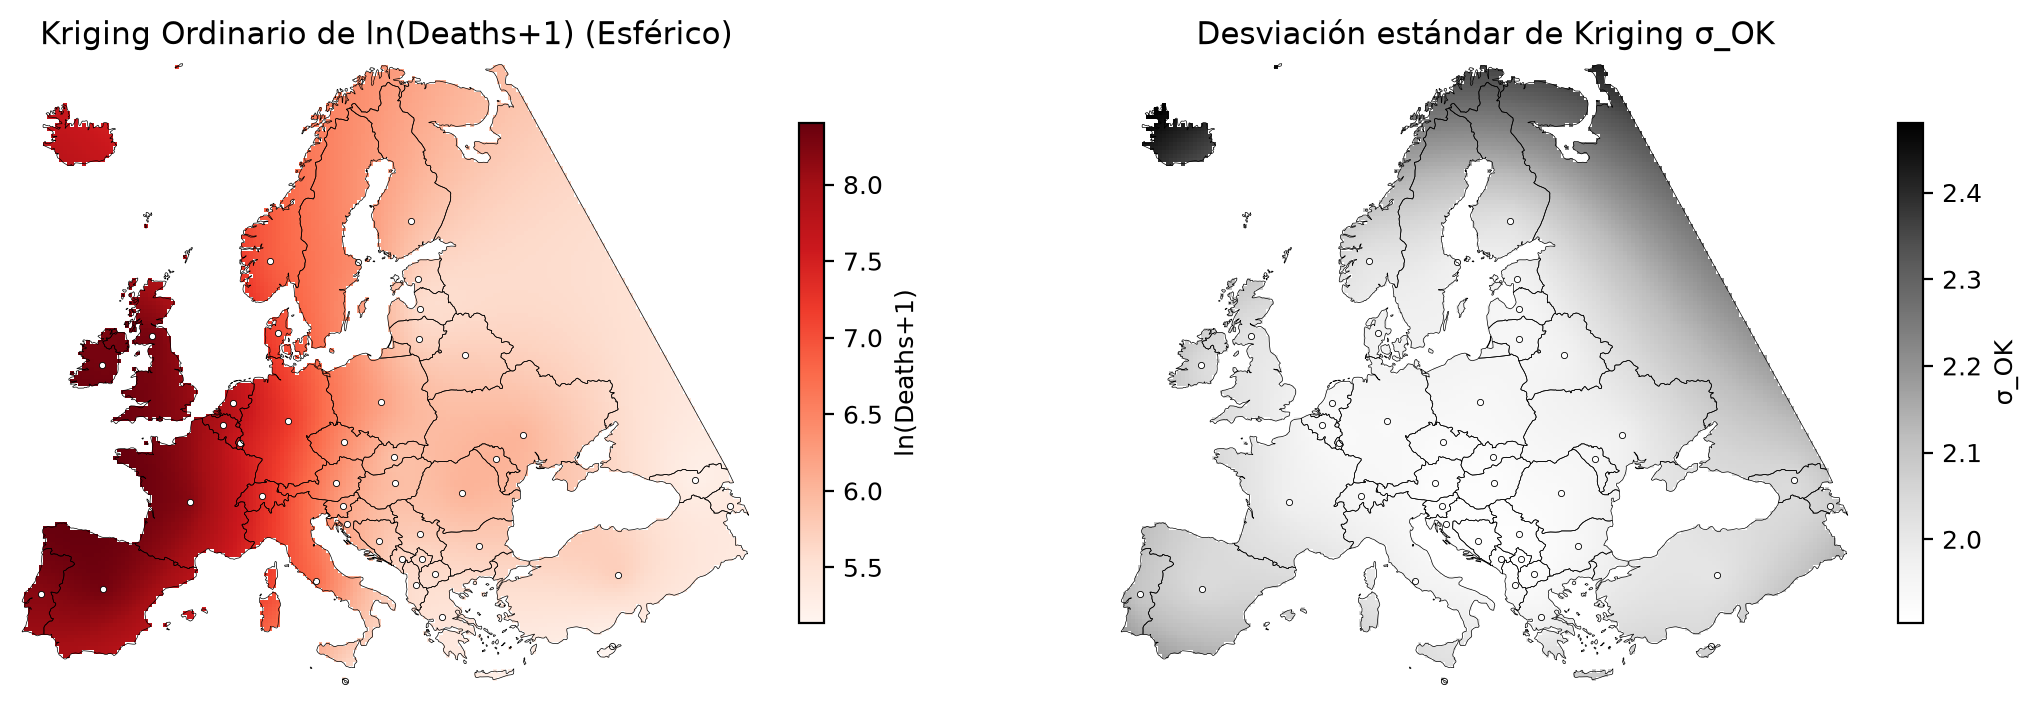
\includegraphics[width=0.85\linewidth]{f3_ok_deaths.png}
\nota{Grilla de 25\,km restringida a superficie terrestre. Los puntos blancos indican los sitios de observación. Elaboración propia.}
\end{figure}

\subsection{Cokriging Ordinario y Semivariograma Cruzado}

Sean $Z_1(s)=\lnC$ la variable primaria y $Z_2(s)=\lnD$ la variable secundaria, observadas en los mismos $n$ sitios, situación denominada muestreo isotópico o de variable secundaria co-localizada. El predictor de Cokriging Ordinario es
\[
\hat Z_1(s_0)=\sum_{i=1}^{n}\lambda_{1i}Z_1(s_i)+\sum_{j=1}^{n}\lambda_{2j}Z_2(s_j),
\]
sujeto a las condiciones de insesgadez $\sum_i\lambda_{1i}=1$ y $\sum_j\lambda_{2j}=0$. La minimización de la varianza del error con los multiplicadores $\mu_1$ y $\mu_2$ conduce al sistema
\[
\begin{pmatrix}\Gamma_{11}&\Gamma_{12}&\mathbf 1&\mathbf 0\\\Gamma_{21}&\Gamma_{22}&\mathbf 0&\mathbf 1\\\mathbf 1^\top&\mathbf 0^\top&0&0\\\mathbf 0^\top&\mathbf 1^\top&0&0\end{pmatrix}
\begin{pmatrix}\bm\lambda_1\\\bm\lambda_2\\\mu_1\\\mu_2\end{pmatrix}=
\begin{pmatrix}\bm\gamma_{11}(s_0)\\\bm\gamma_{21}(s_0)\\1\\0\end{pmatrix},\qquad
\sigma^2_{OCK}(s_0)=\bm\lambda_1^\top\bm\gamma_{11}(s_0)+\bm\lambda_2^\top\bm\gamma_{21}(s_0)+\mu_1.
\]
La dependencia entre ambas variables se describe mediante el semivariograma cruzado y su estimador experimental:
\[
\gamma_{12}(h)=\tfrac12 E\big[(Z_1(s+h)-Z_1(s))(Z_2(s+h)-Z_2(s))\big],
\]
\[
\hat\gamma_{12}(h)=\frac{1}{2|N(h)|}\sum_{N(h)}[z_1(s_i)-z_1(s_j)][z_2(s_i)-z_2(s_j)].
\]
Para garantizar que $\sigma^2_{OCK}\ge0$ en cualquier localización, los semivariogramas directos y cruzado se modelaron conjuntamente mediante un Modelo Lineal de Corregionalización \citep{goulard1992,wackernagel2003}:
\[
\bm\Gamma(h)=\begin{pmatrix}\gamma_{11}(h)&\gamma_{12}(h)\\\gamma_{21}(h)&\gamma_{22}(h)\end{pmatrix}=\mathbf B_0\,g_0(h)+\mathbf B_1\,g_1(h),
\]
donde $g_0$ es el efecto pepita, $g_1$ una estructura de meseta unitaria y alcance común $a$, y $\mathbf B_0$ y $\mathbf B_1$ son matrices de corregionalización semidefinidas positivas. Esta es la condición suficiente de admisibilidad y, en el caso bivariado, equivale a la desigualdad de Cauchy-Schwarz $|b^{(k)}_{12}|\le\sqrt{b^{(k)}_{11}b^{(k)}_{22}}$.

\subsubsection{Ajuste del Modelo Lineal de Corregionalización}

Para mantener la coherencia con el análisis variográfico, se fijaron la estructura gaussiana y el alcance de 393\,km de la variable primaria, y los coeficientes directos se estimaron por MV con alcance fijo. El ajuste libre por WLS del semivariograma cruzado produjo una meseta de 5,10, superior a la cota de Cauchy-Schwarz de 3,73, de modo que el modelo resultante no habría sido admisible y podría haber generado varianzas negativas. Por ello se fijó $b^{(k)}_{12}=\rho\sqrt{b^{(k)}_{11}b^{(k)}_{22}}$, con $\rho=0{,}957$ igual a la correlación co-localizada, estimador de momentos de $C_{12}(0)/\sqrt{C_{11}(0)C_{22}(0)}$. El modelo obtenido es admisible, con autovalores de $\mathbf B_1$ iguales a 0,155 y 7,544 (Tabla~\ref{tab:lmc} y Figura~\ref{fig:lmc}).

\begin{table}[H]\centering\setstretch{1}\small
\caption{Coeficientes del Modelo Lineal de Corregionalización}\label{tab:lmc}
\begin{tabular}{lcc}\toprule
Componente & Efecto pepita ($\mathbf B_0$) & Meseta parcial ($\mathbf B_1$)\\\midrule
$\gamma_{11}$: $\lnC$ & $\approx0$ & 2,899\\
$\gamma_{12}$: semivariograma cruzado & $\approx0$ & 3,570\\
$\gamma_{22}$: $\lnD$ & $\approx0$ & 4,800\\\bottomrule
\end{tabular}
\nota{Estructura gaussiana con alcance práctico común $a=393$\,km. Elaboración propia.}
\end{table}

\begin{figure}[H]
\caption{Semivariogramas Directos y Cruzado Experimentales con el Modelo Lineal de Corregionalización}\label{fig:lmc}
\centering
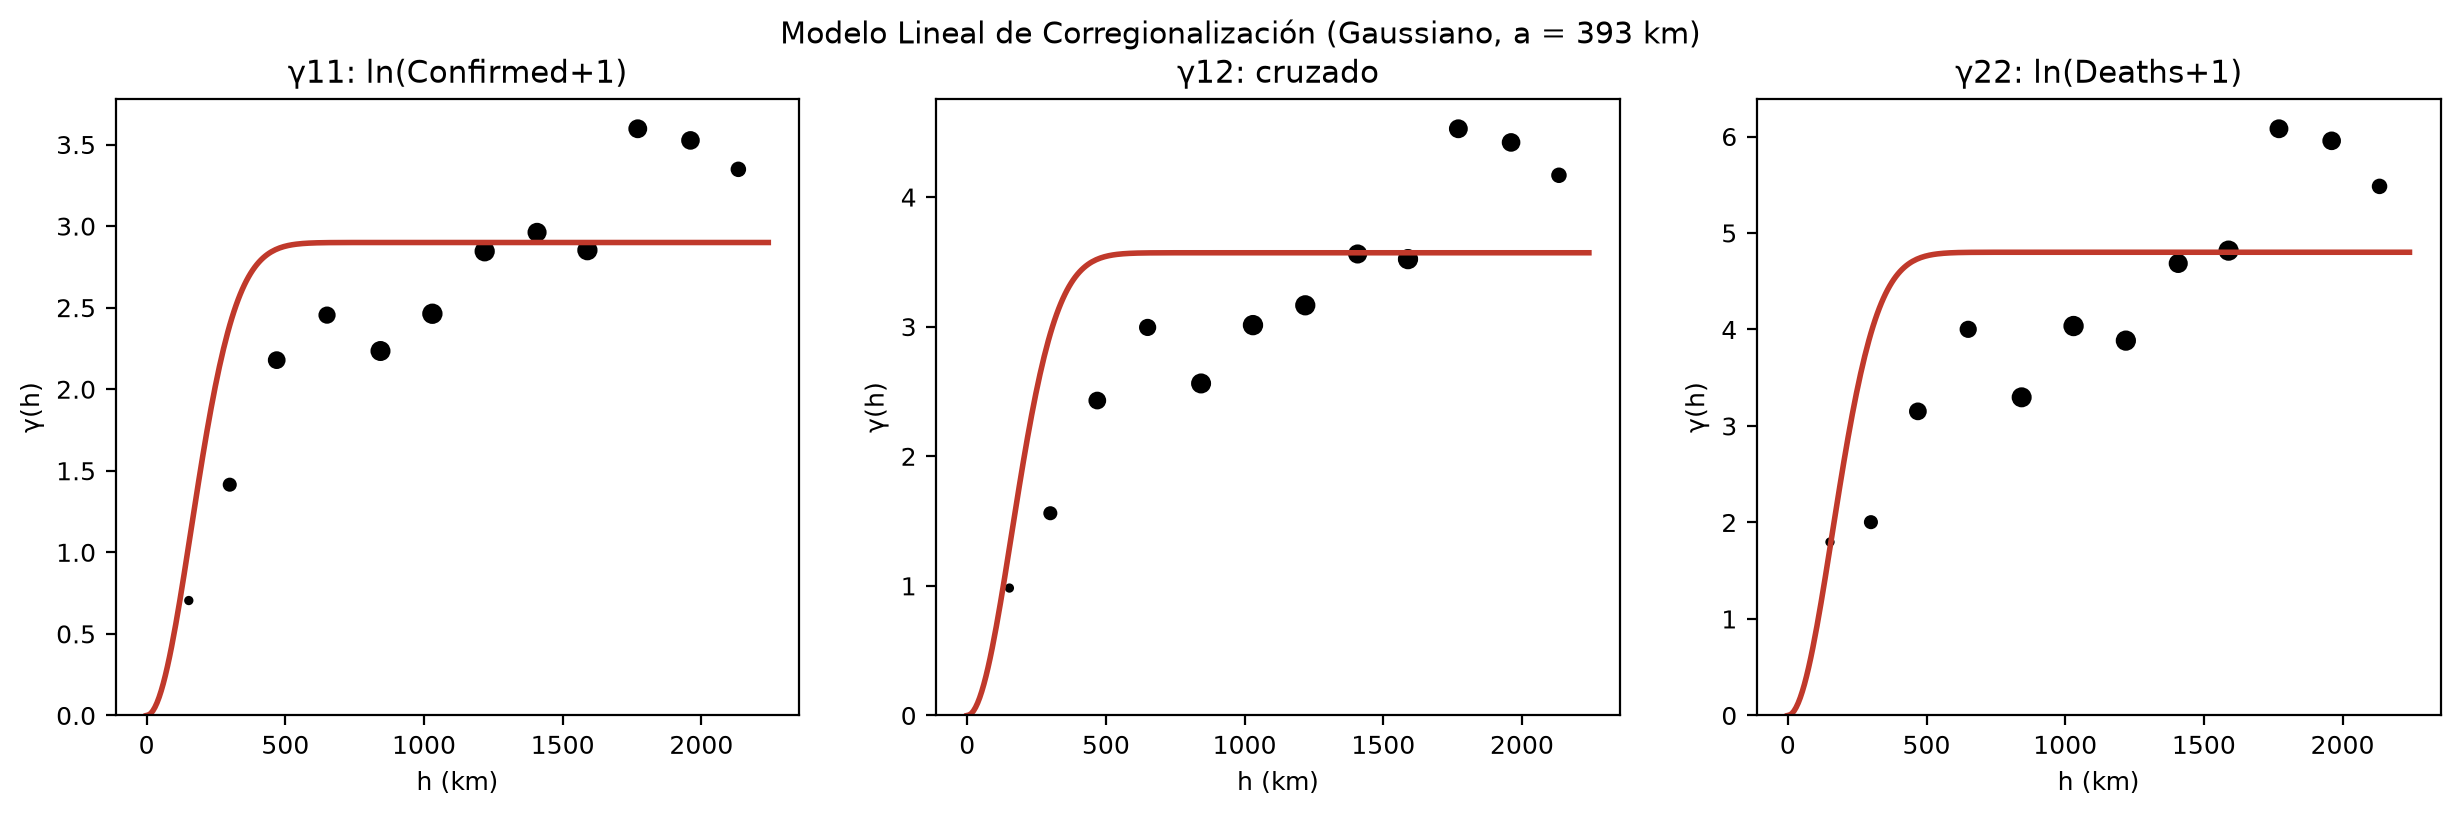
\includegraphics[width=\linewidth]{f3_lmc_variogramas.png}
\nota{Los puntos representan los semivariogramas experimentales y la línea roja, el modelo ajustado. Elaboración propia.}
\end{figure}

Dado que $\mathbf B_0\approx\mathbf 0$ y que la correlación estructural de $\mathbf B_1$ coincide con la co-localizada, el modelo corresponde a una corregionalización intrínseca, $\bm\Gamma(h)=\mathbf V\gamma_u(h)$. Para este caso, en presencia de muestreo isotópico, la teoría establece la propiedad de autokrigeabilidad, según la cual el Cokriging coincide con el Kriging \citep{wackernagel2003}. Los resultados la verifican numéricamente: las superficies de predicción y las varianzas del Kriging Ordinario y del Cokriging Ordinario son idénticas, con una varianza media de 2,197, y las sumas de pesos cumplen $\sum\lambda_{1i}=1$ y $\sum\lambda_{2j}=0$ con precisión de máquina (Figura~\ref{fig:okock}).

\begin{figure}[H]
\caption{Superficies de $\lnC$ por Kriging Ordinario y Cokriging Ordinario y sus Desviaciones Estándar}\label{fig:okock}
\centering
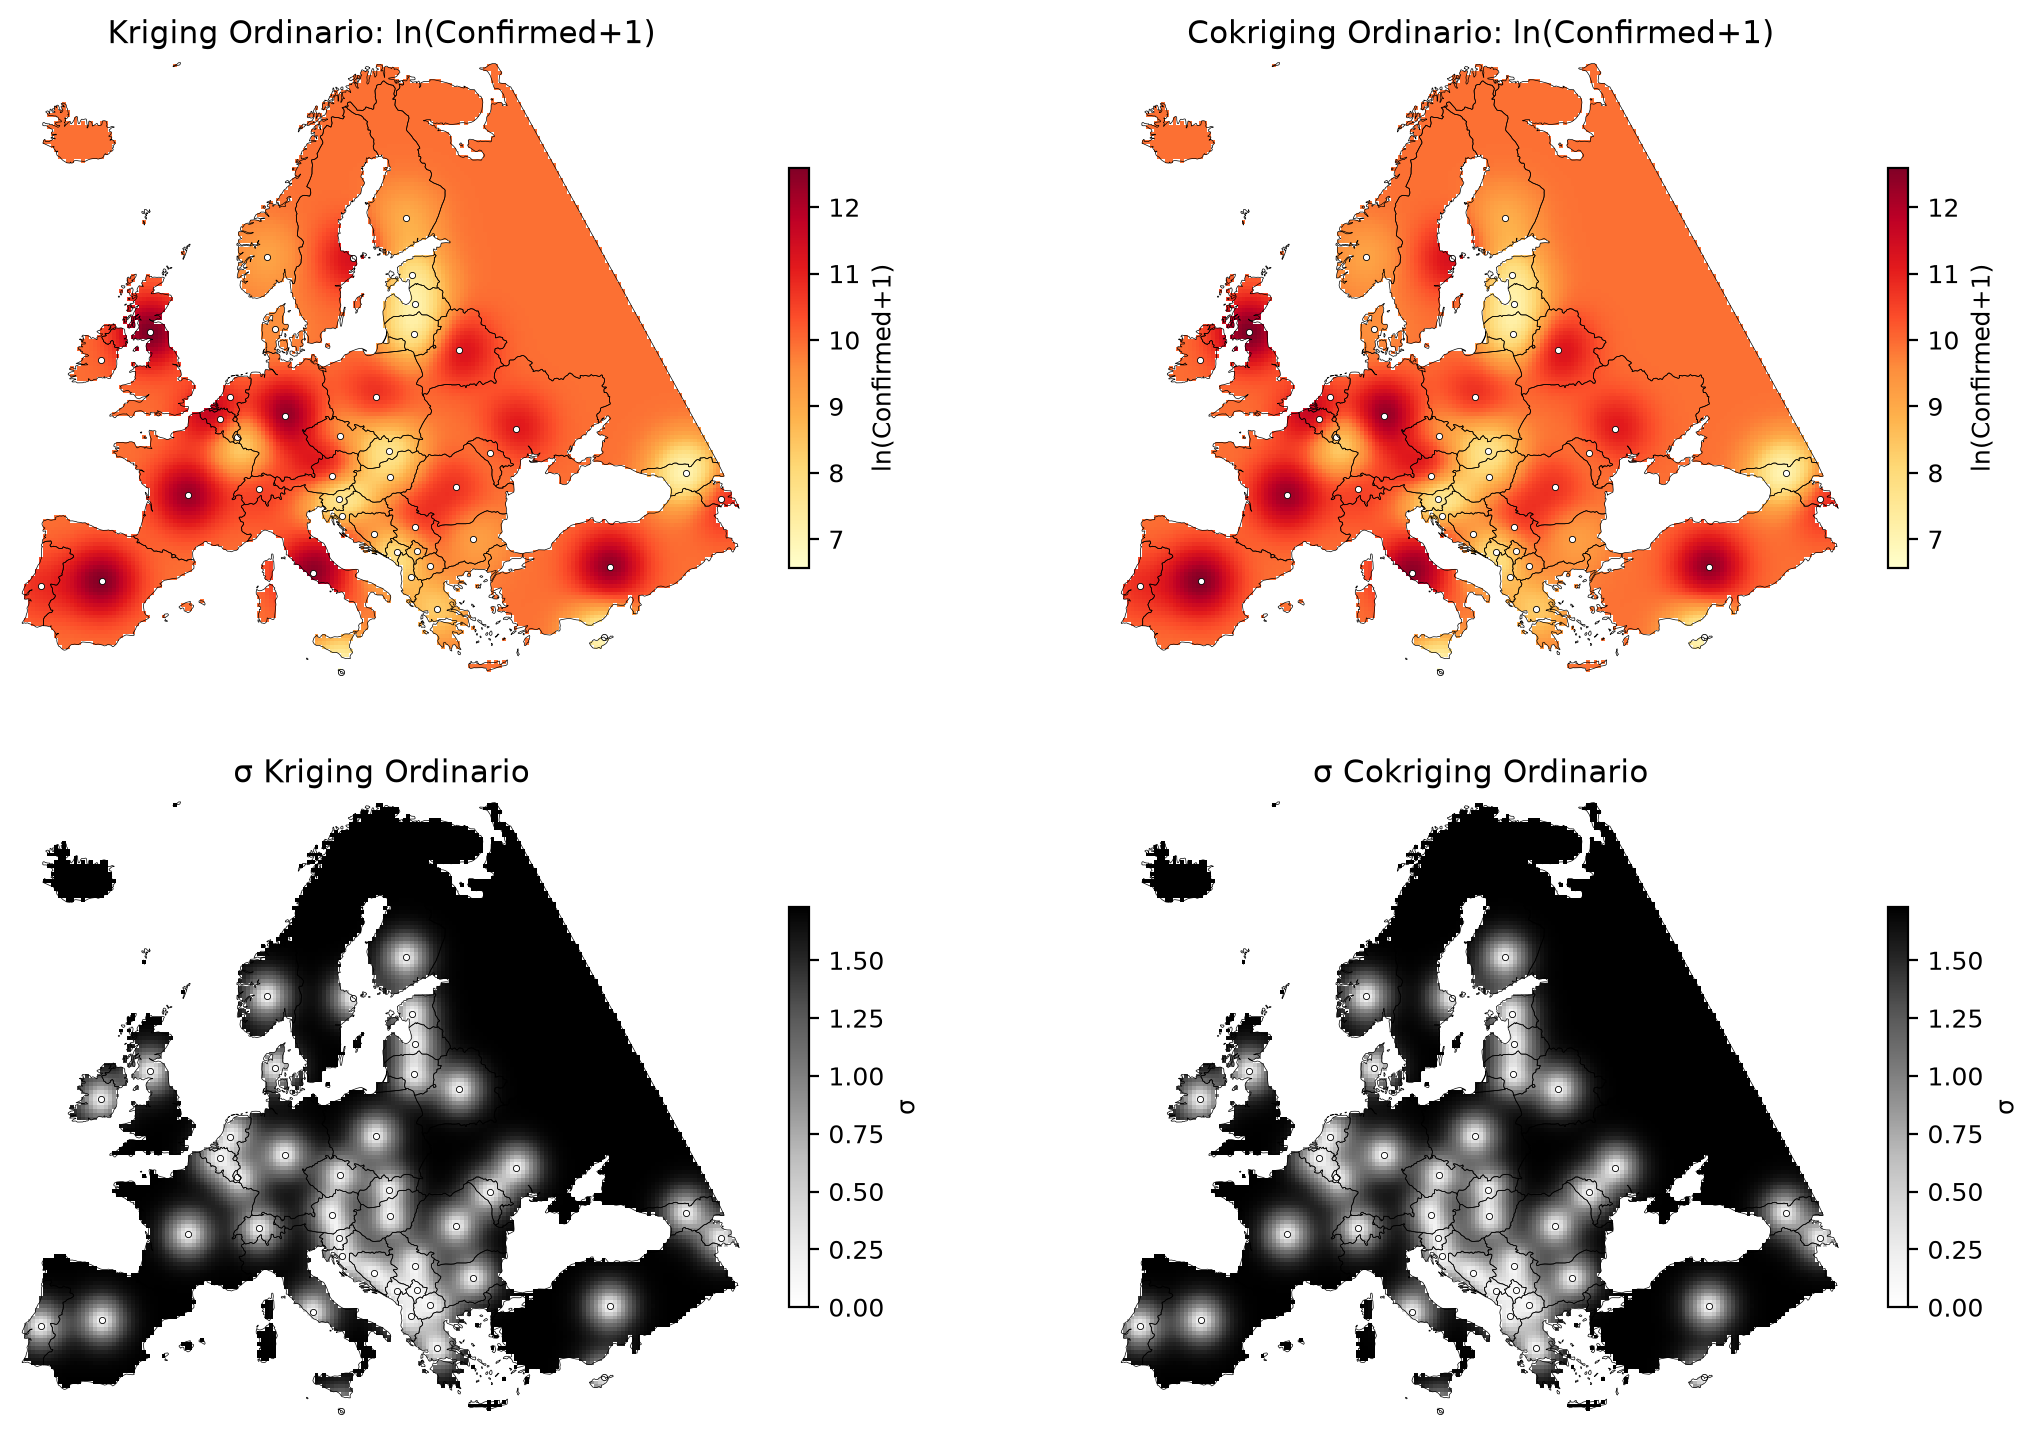
\includegraphics[width=0.92\linewidth]{f3_ok_vs_ock_confirmed.png}
\nota{Fila superior: predicciones; fila inferior: desviaciones estándar del error. Ambas columnas comparten escala de color. Elaboración propia.}
\end{figure}

La superficie estimada concentra la mayor carga en el eje formado por el Reino Unido, el Benelux, Francia y la península ibérica, con focos adicionales en Alemania, Italia, Suecia, Bielorrusia, Ucrania, Rumania y Turquía. Al tratarse de un conteo total, los valores máximos coinciden con los países más poblados y la superficie combina riesgo y tamaño poblacional; por esta razón, en la Fase 4 se incorpora la incidencia por habitante. La desviación estándar es nula en los sitios observados, como corresponde a un interpolador exacto sin efecto pepita, y alcanza la meseta, aproximadamente 1,7, a más de 400\,km de cualquier sitio.

\subsection{Validación Cruzada de los Estimadores}

En la validación cruzada dejando uno fuera se excluye cada sitio $s_k$, se predice su valor con los $n-1$ restantes y se calculan el error $e_k=\hat Z(s_k)-Z(s_k)$ y su versión estandarizada $e_k/\sigma(s_k)$. A partir de ellos se obtienen
\[
\text{RMSE}=\sqrt{\frac1n\sum_{k=1}^n e_k^2},\qquad\text{RMSS}=\sqrt{\frac1n\sum_{k=1}^n\Big(\frac{e_k}{\sigma(s_k)}\Big)^2}.
\]
El RMSE mide la exactitud de la predicción, por lo que se prefieren valores menores. El RMSS mide la calibración de la incertidumbre y su valor ideal es uno: un RMSS mayor que uno indica que el modelo subestima su varianza y produce mapas de incertidumbre optimistas, mientras que un valor menor que uno indica sobrestimación. El error medio y el error medio estandarizado deben ser próximos a cero. La regla de decisión consiste en elegir el estimador de menor RMSE siempre que su RMSS sea cercano a uno y, ante RMSE similares, preferir el de RMSS más próximo a uno \citep{isaaks1989,goovaerts1997}.

Se evaluaron tres escenarios: el Kriging Ordinario; el Cokriging Ordinario isotópico, en el que se excluyen ambas variables en $s_k$ y que representa la predicción en localizaciones sin información; y el Cokriging Ordinario co-localizado, en el que solo se excluye Confirmed y que representa el caso de un territorio con registro confiable de defunciones y subregistro de casos (Tabla~\ref{tab:cv} y Figura~\ref{fig:cv}).

\begin{table}[H]\centering\setstretch{1}\small
\caption{Validación Cruzada de los Estimadores de $\lnC$}\label{tab:cv}
\begin{tabular}{lcccccc}\toprule
Estimador & ME & MAE & RMSE & $r$ & MSE estand. & RMSS\\\midrule
IDW ($p=1{,}5$) & $-0{,}151$ & 1,353 & 1,655 & 0,218 & -- & --\\
Kriging Ordinario (gaussiano, MV) & $-0{,}107$ & 1,276 & 1,583 & 0,360 & $-0{,}043$ & 1,019\\
Cokriging Ordinario isotópico & $-0{,}107$ & 1,276 & 1,583 & 0,360 & $-0{,}043$ & 1,019\\
Cokriging Ordinario co-localizado & $-0{,}023$ & 0,400 & 0,541 & 0,948 & $-0{,}040$ & 1,412\\\bottomrule
\end{tabular}
\nota{$n=42$. Validación cruzada dejando uno fuera. MSE estand. = error medio estandarizado. IDW no produce varianza de predicción, por lo que no admite métricas estandarizadas. Elaboración propia.}
\end{table}

\begin{figure}[H]
\caption{Valores Observados Frente a Predichos en la Validación Cruzada}\label{fig:cv}
\centering
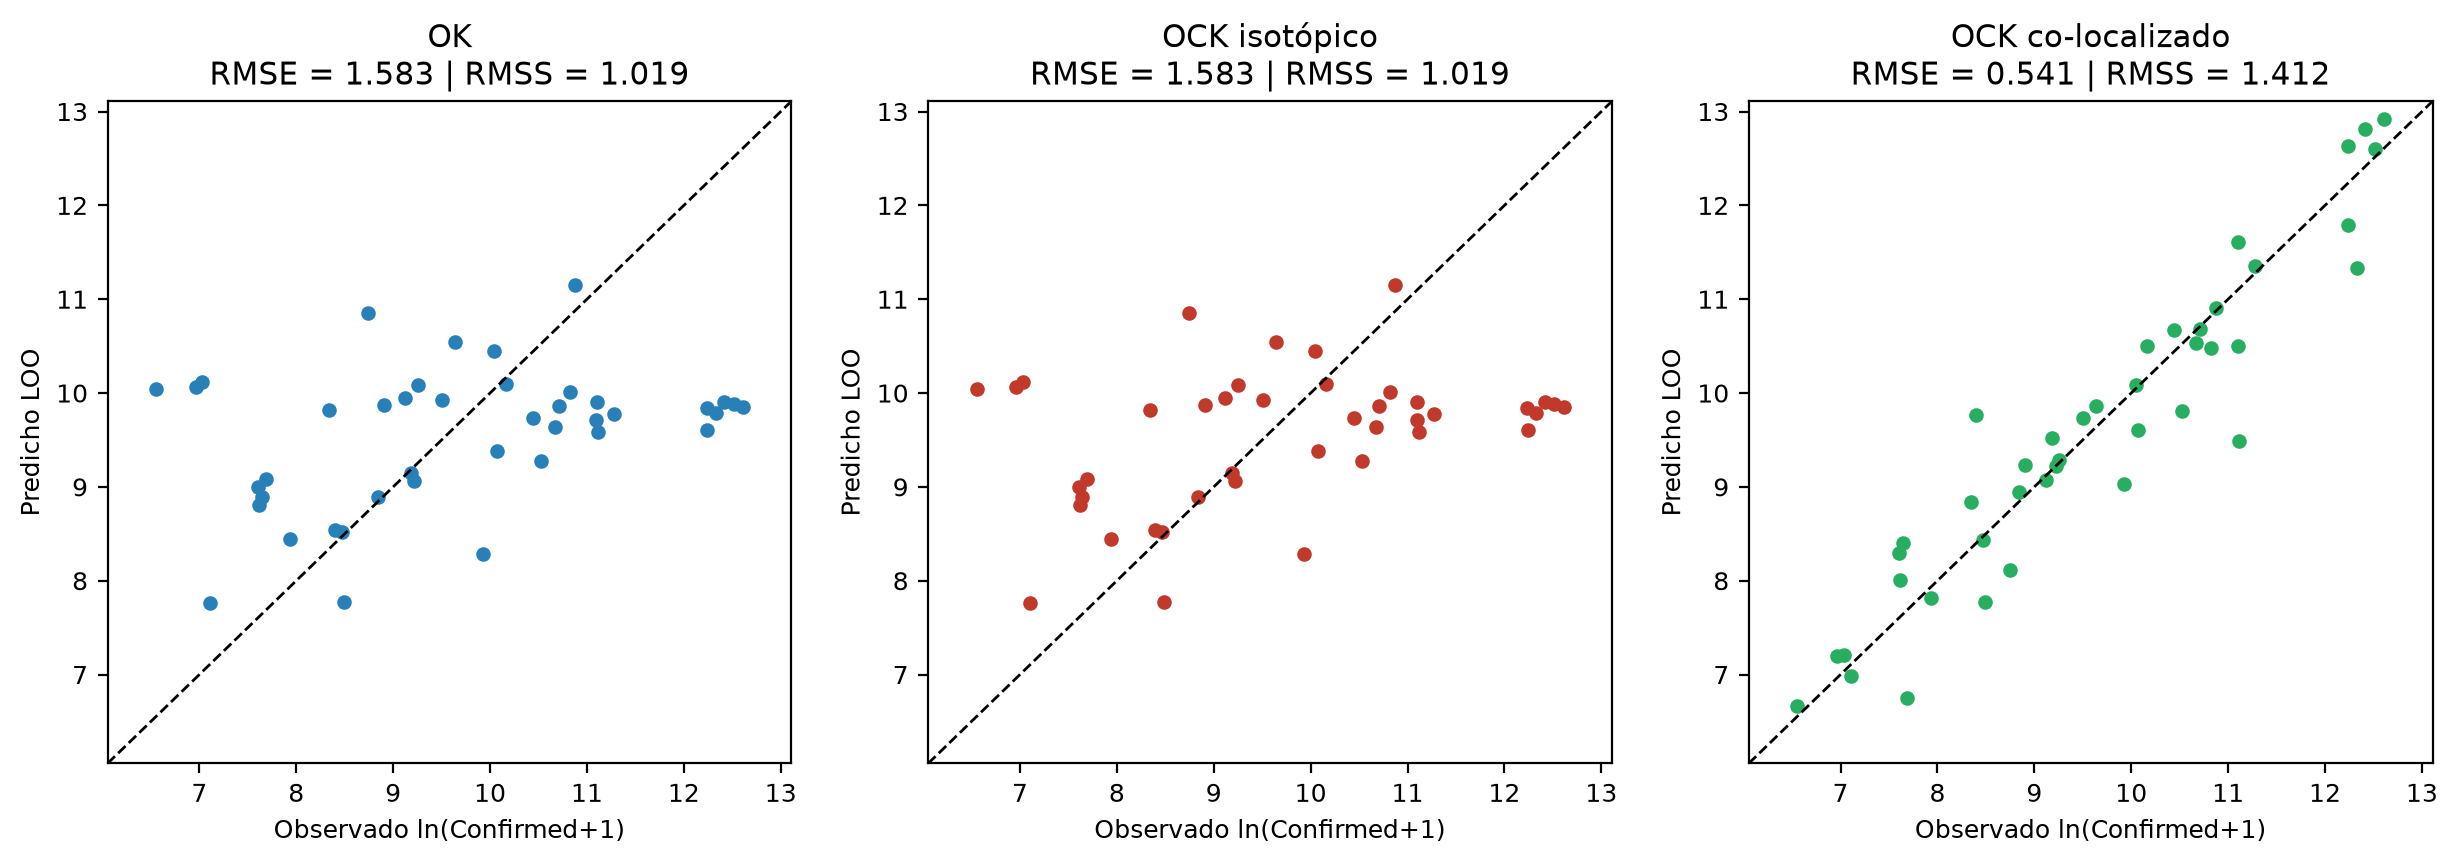
\includegraphics[width=\linewidth]{f3_validacion_cruzada.png}
\nota{La línea discontinua representa la igualdad entre valores observados y predichos. Elaboración propia.}
\end{figure}

El Kriging Ordinario redujo el RMSE en 4,4\,\% respecto del IDW y, a diferencia de este, proporcionó una varianza bien calibrada (RMSS = 1,02) con un sesgo medio próximo a cero. El Cokriging isotópico produjo resultados idénticos a los del Kriging, en concordancia con la propiedad de autokrigeabilidad. La Figura~\ref{fig:cv} muestra, además, el efecto de suavizamiento propio del Kriging, por el cual los valores extremos, correspondientes a países con más de 200\,000 casos, se predicen desplazados hacia la media \citep{goovaerts1997}. Cuando la variable secundaria se conoce en el sitio de predicción, el Cokriging co-localizado redujo el RMSE a 0,541, una disminución de 66\,\%, y elevó la correlación entre valores observados y predichos de 0,36 a 0,95; su RMSS de 1,41 indica, sin embargo, que $\sigma^2_{OCK}$ subestima el error en un factor aproximado de $1{,}41^2\approx2$, por lo que los intervalos de predicción deben ampliarse en esa proporción.

En síntesis, para la cartografía de zonas sin observaciones el Kriging Ordinario y el Cokriging Ordinario resultan equivalentes, y se reporta el Cokriging por incorporar toda la información disponible sin pérdida de exactitud. Cuando la variable secundaria está disponible en la localización de interés, el Cokriging es claramente superior, siempre que su varianza se recalibre.

% =====================================================================
\section{Fase 4: Discusión Territorial y Recomendaciones}
% =====================================================================

Para la formulación de recomendaciones se integraron tres insumos: la superficie del Cokriging Ordinario y su desviación estándar $\sigma_{OCK}$; una superficie complementaria de incidencia por 100\,000 habitantes estimada por Kriging Ordinario, con un semivariograma esférico sin efecto pepita y alcance de 461\,km (RMSE = 0,839; RMSS = 0,98), que corrige el efecto del tamaño poblacional; y los indicadores de capacidad sanitaria de Our World in Data. Se definieron como zonas de alta carga el quintil superior de cada superficie, es decir, valores del Cokriging iguales o superiores a 35\,147 casos acumulados o incidencias iguales o superiores a 280 casos por 100\,000 habitantes (Figura~\ref{fig:f4}).

\begin{figure}[H]
\caption{Zonas de Alta Carga, Incidencia Predicha e Incertidumbre del Cokriging Ordinario}\label{fig:f4}
\centering
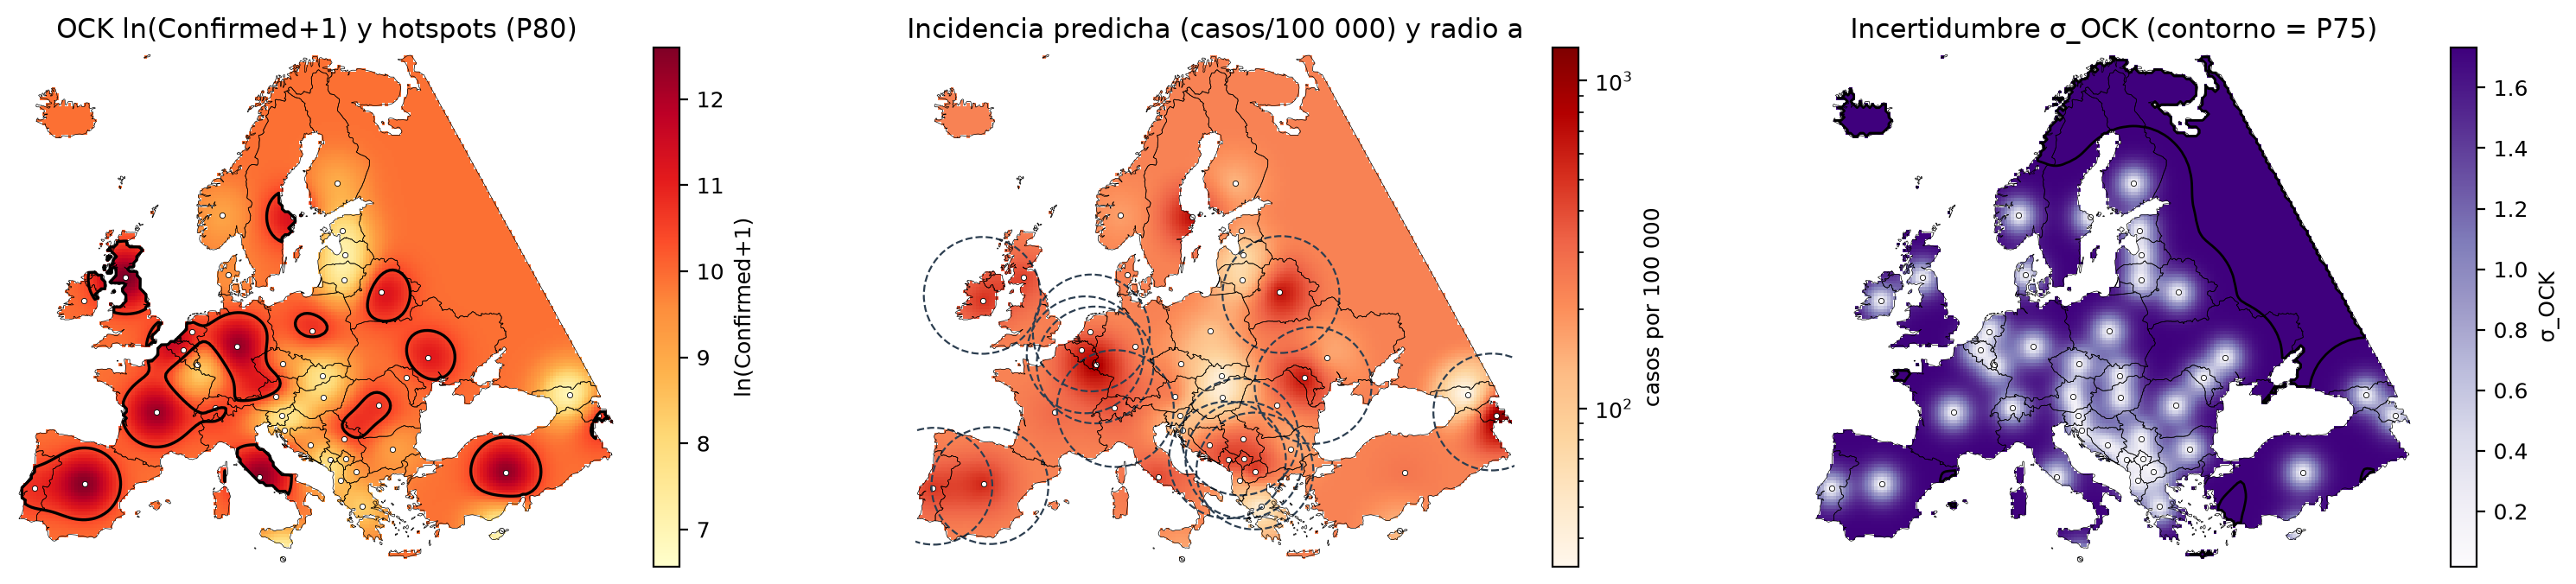
\includegraphics[width=\linewidth]{f4_hotspots_incertidumbre.png}
\nota{Izquierda: superficie del Cokriging con el contorno del percentil 80. Centro: incidencia predicha con círculos de radio $a=461$\,km alrededor de los países de alto riesgo. Derecha: desviación estándar $\sigma_{OCK}$ con el contorno del percentil 75. Elaboración propia a partir de \citet{dong2020}, \citet{owid2020} y \citet{naturalearth}.}
\end{figure}

\subsection{Recomendaciones Cuantitativas}

\subsubsection{Refuerzo de la Capacidad Hospitalaria en Zonas de Alta Carga}

Ocho países presentan al menos la mitad de su territorio en zona de alta carga y una dotación de camas hospitalarias inferior a la mediana del área de estudio, de 4,50 camas por cada 1000 habitantes. El déficit, calculado como $(4{,}50-\text{camas})\times\text{población}/1000$, asciende a 247\,407 camas (Tabla~\ref{tab:r1}). El 83\,\% de dicho déficit se concentra en el Reino Unido y España, países en los que, además, más del 18\,\% de la población tiene 65 años o más, grupo de mayor letalidad. Se recomienda priorizar la redistribución de camas, personal y equipamiento de cuidados intensivos en ese orden, comenzando por la península ibérica y las islas británicas.

\begin{table}[H]\centering\setstretch{1}\small
\caption{Déficit de Camas Hospitalarias en los Países de Alta Carga con Dotación Inferior a la Mediana}\label{tab:r1}
\begin{tabularx}{\linewidth}{>{\raggedright\arraybackslash}p{3.3cm}*{5}{>{\centering\arraybackslash}X}}\toprule
País & Alta carga, casos (\%) & Alta carga, incidencia (\%) & Camas por 1000 hab. & Población $\geq$ 65 años (\%) & Déficit de camas\\\midrule
Reino Unido & 56,6 & 45,2 & 2,54 & 18,5 & 132\,655\\
España & 53,7 & 52,4 & 2,97 & 19,4 & 73\,003\\
Países Bajos & 76,3 & 61,0 & 3,32 & 18,8 & 20\,813\\
Portugal & 72,5 & 94,9 & 3,39 & 21,5 & 11\,452\\
Irlanda & 11,9 & 100,0 & 2,96 & 13,9 & 7\,761\\
Armenia & 29,3 & 90,2 & 4,20 & 11,2 & 848\\
Macedonia del Norte & 0,0 & 80,0 & 4,28 & 13,3 & 471\\
Montenegro & 0,0 & 100,0 & 3,86 & 14,8 & 405\\\midrule
Total & & & & & 247\,407\\\bottomrule
\end{tabularx}
\nota{Los porcentajes de alta carga indican la proporción del territorio nacional situada en el quintil superior de la superficie correspondiente. La mediana de camas del área de estudio es 4,50 por cada 1000 habitantes. Elaboración propia a partir de \citet{owid2020}.}
\end{table}

\subsubsection{Densificación de la Red de Vigilancia en Zonas de Alta Incertidumbre}

El 25\,\% del territorio presenta una desviación estándar $\sigma_{OCK}\ge1{,}73$, correspondiente al cuartil superior. Este nivel de incertidumbre se alcanza cuando el sitio de reporte más próximo se encuentra a más de 450\,km, distancia del mismo orden que el alcance del semivariograma. Las zonas críticas son la Rusia europea, con el 74\,\% de su superficie en esta condición, Noruega (39\,\%), Suecia (33\,\%) y Finlandia (30\,\%). Se recomienda establecer reportes a escala subnacional con al menos un punto de vigilancia por cada celda de aproximadamente 450 por 450\,km, equivalente a 200\,000\,km², lo que implica alrededor de once puntos en la Rusia europea, tres en Suecia y dos en Noruega y en Finlandia. Esta densificación reduciría $\sigma_{OCK}$ por debajo del umbral en toda la región y corregiría el muestreo preferencial identificado en la Fase 2.

\subsubsection{Coordinación de Medidas Territoriales en el Radio de Dependencia Espacial}

El semivariograma de la incidencia carece de efecto pepita y presenta un alcance práctico de 461\,km, distancia dentro de la cual la incidencia de un país aporta información sobre la de sus vecinos. En torno a los 14 países de alto riesgo, a saber, España, Portugal, los Países Bajos, Bélgica, Luxemburgo, Suiza, Irlanda, Bielorrusia, Moldavia, Armenia, Serbia, Kosovo, Macedonia del Norte y Montenegro, se recomienda acordar en bloque las medidas territoriales con los 14 países situados dentro de dicho radio, entre ellos Francia, Alemania, el Reino Unido, Rumania, Ucrania, Grecia, Bulgaria, Hungría y los Balcanes occidentales. Tales medidas comprenden controles sanitarios en frontera, restricción de la movilidad no esencial e intercambio de información en tiempo real. La adopción de decisiones país por país ignora la dependencia espacial estimada.

% =====================================================================
\section{Discusión}
% =====================================================================

Los resultados deben valorarse a la luz de cinco limitaciones. En primer lugar, cada observación corresponde al centroide de un país, por lo que las superficies interpolan agregados de área y no deben leerse como riesgo individual ni subnacional; esta situación expone el análisis a la falacia ecológica y al problema de la unidad de área modificable \citep{openshaw1984,gotway2002}, que podrían abordarse mediante un Kriging de área a punto con datos subnacionales. En segundo lugar, las diferencias entre países en la capacidad diagnóstica, la definición de caso y el registro de defunciones se suman a la variabilidad a microescala; el efecto pepita nulo estimado por máxima verosimilitud podría subestimarla, dado que la distancia mínima entre centroides limita la información disponible sobre el semivariograma en las proximidades del origen.

En tercer lugar, con 42 observaciones las primeras clases de distancia contienen pocos pares (11 y 33), razón por la cual la selección del modelo se fundamentó en la validación cruzada y no únicamente en el ajuste gráfico. En cuarto lugar, la Federación de Rusia, cuyo centroide se sitúa fuera de la ventana de estudio, no aporta observaciones, lo que explica la elevada incertidumbre en el este del continente. Por último, el análisis es de carácter transversal; su extensión natural consiste en un modelo espacio-temporal que aproveche la serie completa \citep{cressie2011}.

% =====================================================================
\section{Conclusiones}
% =====================================================================

La proyección de los datos constituye un requisito para el análisis geoestadístico: las distancias calculadas en grados presentaron un error mediano de 29,9\,\% y máximo de 125,9\,\%, frente a un error máximo inferior a 2,1\,\% en EPSG:3035. El corte temporal al 26 de julio de 2020 definió una única realización del campo aleatorio, y la transformación $\ln(x+1)$ redujo la asimetría de 2,21 a $-0{,}39$ y restituyó la normalidad de la variable. La homogeneización del soporte, mediante la exclusión de las ubicaciones con menos de 500\,000 habitantes, fue la decisión metodológica de mayor impacto, al reducir la proporción pepita/meseta de 61,7\,\% a 23,3\,\% con mínimos cuadrados ponderados y a valores próximos a cero con máxima verosimilitud.

Los sitios de reporte no siguen un patrón de Completa Aleatoriedad Espacial: son regulares a escala corta, por inhibición político-administrativa, y agregados a escala larga, por la existencia de amplios espacios sin observaciones en el este. El atributo presentó un conglomerado de alta incidencia en el litoral atlántico y un conglomerado de baja incidencia en Europa central. La dependencia espacial de los casos confirmados es fuerte, con un modelo gaussiano sin efecto pepita y un alcance de 393\,km, y el Kriging Ordinario superó al interpolador IDW con una varianza adecuadamente calibrada.

Bajo corregionalización intrínseca y muestreo isotópico, el Cokriging Ordinario coincidió con el Kriging Ordinario, mientras que con la variable secundaria co-localizada redujo el error cuadrático medio en 66\,\%, aunque requiere recalibrar su varianza. Las superficies estimadas y su incertidumbre permitieron cuantificar un déficit de aproximadamente 247\,400 camas en ocho países de alta carga, establecer un espaciamiento máximo de 450\,km para la red de vigilancia y delimitar un radio de coordinación territorial de 461\,km.


\clearpage
\begin{thebibliography}{99}

\bibitem[Annoni et~al.(2003)]{annoni2003} Annoni, A., Luzet, C., Gubler, E., \& Ihde, J. (Eds.). (2003). \emph{Map projections for Europe} (EUR 20120 EN). European Commission, Joint Research Centre.

\bibitem[Anselin(1995)]{anselin1995} Anselin, L. (1995). Local indicators of spatial association: LISA. \emph{Geographical Analysis, 27}(2), 93--115. \url{https://doi.org/10.1111/j.1538-4632.1995.tb00338.x}

\bibitem[Baddeley et~al.(2015)]{baddeley2015} Baddeley, A., Rubak, E., \& Turner, R. (2015). \emph{Spatial point patterns: Methodology and applications with R}. CRC Press.

\bibitem[Cambardella et~al.(1994)]{cambardella1994} Cambardella, C. A., Moorman, T. B., Novak, J. M., Parkin, T. B., Karlen, D. L., Turco, R. F., \& Konopka, A. E. (1994). Field-scale variability of soil properties in central Iowa soils. \emph{Soil Science Society of America Journal, 58}(5), 1501--1511.

\bibitem[Chilès y Delfiner(2012)]{chiles2012} Chilès, J.-P., \& Delfiner, P. (2012). \emph{Geostatistics: Modeling spatial uncertainty} (2.ª ed.). Wiley.

\bibitem[Clark y Evans(1954)]{clark1954} Clark, P. J., \& Evans, F. C. (1954). Distance to nearest neighbor as a measure of spatial relationships in populations. \emph{Ecology, 35}(4), 445--453.

\bibitem[Cressie(1985)]{cressie1985} Cressie, N. (1985). Fitting variogram models by weighted least squares. \emph{Mathematical Geology, 17}(5), 563--586.

\bibitem[Cressie(1993)]{cressie1993} Cressie, N. (1993). \emph{Statistics for spatial data} (ed. rev.). Wiley.

\bibitem[Cressie y Wikle(2011)]{cressie2011} Cressie, N., \& Wikle, C. K. (2011). \emph{Statistics for spatio-temporal data}. Wiley.

\bibitem[Diggle(1985)]{diggle1985} Diggle, P. J. (1985). A kernel method for smoothing point process data. \emph{Journal of the Royal Statistical Society: Series C (Applied Statistics), 34}(2), 138--147.

\bibitem[Diggle(2013)]{diggle2013} Diggle, P. J. (2013). \emph{Statistical analysis of spatial and spatio-temporal point patterns} (3.ª ed.). CRC Press.

\bibitem[Diggle et~al.(2010)]{diggle2010} Diggle, P. J., Menezes, R., \& Su, T. (2010). Geostatistical inference under preferential sampling. \emph{Journal of the Royal Statistical Society: Series C (Applied Statistics), 59}(2), 191--232.

\bibitem[Diggle et~al.(1998)]{diggle1998} Diggle, P. J., Tawn, J. A., \& Moyeed, R. A. (1998). Model-based geostatistics. \emph{Journal of the Royal Statistical Society: Series C (Applied Statistics), 47}(3), 299--350. \url{https://doi.org/10.1111/1467-9876.00113}

\bibitem[Dong et~al.(2020)]{dong2020} Dong, E., Du, H., \& Gardner, L. (2020). An interactive web-based dashboard to track COVID-19 in real time. \emph{The Lancet Infectious Diseases, 20}(5), 533--534. \url{https://doi.org/10.1016/S1473-3099(20)30120-1}

\bibitem[Getis y Ord(1992)]{getis1992} Getis, A., \& Ord, J. K. (1992). The analysis of spatial association by use of distance statistics. \emph{Geographical Analysis, 24}(3), 189--206.

\bibitem[Goovaerts(1997)]{goovaerts1997} Goovaerts, P. (1997). \emph{Geostatistics for natural resources evaluation}. Oxford University Press.

\bibitem[Gotway y Young(2002)]{gotway2002} Gotway, C. A., \& Young, L. J. (2002). Combining incompatible spatial data. \emph{Journal of the American Statistical Association, 97}(458), 632--648.

\bibitem[Goulard y Voltz(1992)]{goulard1992} Goulard, M., \& Voltz, M. (1992). Linear coregionalization model: Tools for estimation and choice of cross-variogram matrix. \emph{Mathematical Geology, 24}(3), 269--286.

\bibitem[Isaaks y Srivastava(1989)]{isaaks1989} Isaaks, E. H., \& Srivastava, R. M. (1989). \emph{An introduction to applied geostatistics}. Oxford University Press.

\bibitem[Journel(1980)]{journel1980} Journel, A. G. (1980). The lognormal approach to predicting local distributions of selective mining unit grades. \emph{Mathematical Geology, 12}(4), 285--303.

\bibitem[Journel y Huijbregts(1978)]{journel1978} Journel, A. G., \& Huijbregts, C. J. (1978). \emph{Mining geostatistics}. Academic Press.

\bibitem[Matheron(1963)]{matheron1963} Matheron, G. (1963). Principles of geostatistics. \emph{Economic Geology, 58}(8), 1246--1266.

\bibitem[Mathieu et~al.(2020)]{owid2020} Mathieu, E., Ritchie, H., Rodés-Guirao, L., Appel, C., Giattino, C., Hasell, J., Macdonald, B., Dattani, S., Beltekian, D., Ortiz-Ospina, E., \& Roser, M. (2020). \emph{Coronavirus pandemic (COVID-19)}. Our World in Data. \url{https://ourworldindata.org/coronavirus}

\bibitem[Moran(1950)]{moran1950} Moran, P. A. P. (1950). Notes on continuous stochastic phenomena. \emph{Biometrika, 37}(1/2), 17--23.

\bibitem[Natural Earth(s.f.)]{naturalearth} Natural Earth. (s.f.). \emph{Admin 0: Countries, 1:50m cultural vectors}. \url{https://www.naturalearthdata.com}

\bibitem[Openshaw(1984)]{openshaw1984} Openshaw, S. (1984). \emph{The modifiable areal unit problem}. Geo Books.

\bibitem[Patterson y Thompson(1971)]{patterson1971} Patterson, H. D., \& Thompson, R. (1971). Recovery of inter-block information when block sizes are unequal. \emph{Biometrika, 58}(3), 545--554.

\bibitem[Rey y Anselin(2007)]{rey2007} Rey, S. J., \& Anselin, L. (2007). PySAL: A Python library of spatial analytical methods. \emph{The Review of Regional Studies, 37}(1), 5--27.

\bibitem[Ripley(1976)]{ripley1976} Ripley, B. D. (1976). The second-order analysis of stationary point processes. \emph{Journal of Applied Probability, 13}(2), 255--266.

\bibitem[Shepard(1968)]{shepard1968} Shepard, D. (1968). A two-dimensional interpolation function for irregularly-spaced data. En \emph{Proceedings of the 1968 23rd ACM National Conference} (pp. 517--524). ACM.

\bibitem[Silverman(1986)]{silverman1986} Silverman, B. W. (1986). \emph{Density estimation for statistics and data analysis}. Chapman \& Hall.

\bibitem[Snyder(1987)]{snyder1987} Snyder, J. P. (1987). \emph{Map projections: A working manual} (U.S. Geological Survey Professional Paper 1395). U.S. Government Printing Office.

\bibitem[Stein(1999)]{stein1999} Stein, M. L. (1999). \emph{Interpolation of spatial data: Some theory for kriging}. Springer.

\bibitem[Tobler(1970)]{tobler1970} Tobler, W. R. (1970). A computer movie simulating urban growth in the Detroit region. \emph{Economic Geography, 46}(sup1), 234--240.

\bibitem[van Lieshout y Baddeley(1996)]{vanlieshout1996} van Lieshout, M. N. M., \& Baddeley, A. J. (1996). A nonparametric measure of spatial interaction in point patterns. \emph{Statistica Neerlandica, 50}(3), 344--361.

\bibitem[Wackernagel(2003)]{wackernagel2003} Wackernagel, H. (2003). \emph{Multivariate geostatistics: An introduction with applications} (3.ª ed.). Springer.

\bibitem[Webster y Oliver(2007)]{webster2007} Webster, R., \& Oliver, M. A. (2007). \emph{Geostatistics for environmental scientists} (2.ª ed.). Wiley.

\end{thebibliography}

\clearpage
\begin{center}\textbf{Apéndice A}\\\textbf{Correspondencia Entre los Ítems de la Práctica y las Secciones del Informe}\end{center}

\begin{table}[H]\centering\setstretch{1}\small
\caption{Ubicación del Desarrollo de Cada Ítem de la Práctica}\label{tab:items}
\begin{tabularx}{\linewidth}{lX}\toprule
Ítem & Sección del informe\\\midrule
1.1 a) & Fase 1: Sesgo de la Distancia Euclidiana en Coordenadas Geográficas\\
1.1 b) & Fase 1: Sistema de Coordenadas Proyectadas Propuesto\\
1.2 a) & Fase 1: Corte Temporal\\
1.2 b) & Fase 1: Transformación Logarítmica de los Casos Confirmados\\
2.1 a) & Fase 2: Estimación de Densidad Kernel y Ancho de Banda\\
2.1 b) & Fase 2: Contraste de Completa Aleatoriedad Espacial\\
2.2 a) & Fase 2: Formulación del Interpolador por Inverso de la Distancia\\
2.2 b) & Fase 2: Efecto del Parámetro de Potencia y Limitaciones del Método\\
3.1 a) & Fase 3: Semivariograma Experimental y Parámetros Estructurales\\
3.1 b) & Fase 3: Modelos Teóricos de Semivariograma\\
3.2 a) & Fase 3: Sistema del Kriging Ordinario para las Defunciones\\
3.2 b) & Fase 3: Cokriging Ordinario y Semivariograma Cruzado\\
3.2 c) & Fase 3: Validación Cruzada de los Estimadores\\
4.1 & Fase 4: Recomendaciones Cuantitativas\\\bottomrule
\end{tabularx}
\nota{Las secciones adicionales sobre homogeneización del soporte, autocorrelación del atributo, Kriging Universal y ajuste del Modelo Lineal de Corregionalización complementan los ítems solicitados. Elaboración propia.}
\end{table}

\clearpage
\begin{center}\textbf{Apéndice B}\\\textbf{Reproducibilidad del Análisis}\end{center}

El análisis completo se encuentra en el cuaderno Jupyter \texttt{PC2\_Grupo6.ipynb}, que se ejecuta de principio a fin, lee \emph{Data Spatial} directamente desde GitHub y descarga una sola vez las fuentes externas, que almacena recortadas. Los parámetros principales fueron los siguientes: fecha de corte, 26 de julio de 2020; ventana geográfica entre 25\,°O y 46\,°E y entre 34\,°N y 72\,°N; sistema de referencia EPSG:3035 con coordenadas en kilómetros; grilla de predicción de 25\,km, con 14\,167 nodos sobre superficie terrestre; umbral de soporte de 500\,000 habitantes; 199 simulaciones para las envolventes de Completa Aleatoriedad Espacial; 999 permutaciones para los índices de Moran, LISA y $G_i^*$; validación cruzada dejando uno fuera; y semilla aleatoria 2020. La implementación propia del Kriging Ordinario se verificó contra la biblioteca \texttt{pykrige}, con una diferencia máxima en la predicción inferior a $10^{-4}$. La organización de los archivos se describe en la Tabla~\ref{tab:archivos}.

\begin{table}[H]\centering\setstretch{1}\small
\caption{Estructura de Archivos del Proyecto}\label{tab:archivos}
\begin{tabularx}{\linewidth}{lX}\toprule
Ruta & Contenido\\\midrule
\texttt{PC2\_Grupo6.ipynb} & Cuaderno con las cuatro fases: fundamentos, código y resultados ejecutados\\
\texttt{data/} & Copia de respaldo de \texttt{Data Spatial.csv} (la fuente principal es GitHub), recorte de Our World in Data y fronteras de Natural Earth\\
\texttt{figuras/} & Figuras en formato PNG a 200 puntos por pulgada\\
\texttt{resultados/} & Tablas CSV de cada fase, puntos con predicciones (GeoJSON) y superficies de la grilla (NPZ)\\
\texttt{latex/} & Fuente y versión PDF del presente informe\\\bottomrule
\end{tabularx}
\nota{Elaboración propia.}
\end{table}

\end{document}
